% LTeX: language=en-GB
\documentclass{tudelft-report}

\usepackage[italian,british]{babel}

%% Set up the bibliography
\usepackage[style=ieee, backend=biber]{biblatex}
\addbibresource{report.bib}

%% Additional packages and commands
\usepackage{parskip}
\setlist{itemsep=-2pt} % Reducing white space in lists slightly
\renewcommand{\deg}{\si{\degree}\xspace} % Use \deg easily, everywhere
\usepackage{pdflscape} % Single landscape pages (rotated in the PDF viewer too)
% Draft highlighting: \hl{text to revise}
\usepackage{soul}
\sethlcolor{yellow}
\soulregister{\cite}{7} % Allow \cite and \ref inside \hl{}
\soulregister{\ref}{7}
% \renewcommand{\hl}[1]{#1} % Uncomment to hide all highlights (final version)
% Thesis version: \confidentialtrue = full, strictly confidential version (never disclosed)
%                 \confidentialfalse = public version with modified data (TU Delft repository)
% Usage: \ifconfidential <full-version content> \else <public-version content> \fi
\newif\ifconfidential
\confidentialtrue
% Ragged-right column, width given as a fraction of the line width: P{0.25}
\newcolumntype{P}[1]{>{\raggedright\arraybackslash}p{\dimexpr#1\linewidth-2\tabcolsep\relax}}
\usepackage[most]{tcolorbox}
\definecolor{title}{HTML}{4884d6} % Defined here too so the box colour is available before the cover
% Usage: \begin{objectivebox}{Box title} ... \end{objectivebox}
%        optional tcolorbox keys first: \begin{objectivebox}[colframe=red]{Box title}
\newtcolorbox{objectivebox}[2][]{
  enhanced, breakable,
  parbox=false,             % keep the document's paragraph/list spacing (parskip) inside the box
  title={#2},
  colframe=title!60!black,  % frame + title band (darker blue)
  colback=title!4,          % very light blue body
  coltitle=white,
  fonttitle=\sffamily\large,
  halign title=center,
  boxrule=1.2pt, titlerule=0pt,
  arc=2mm,
  left=10pt, right=10pt, top=8pt, bottom=8pt,
  toptitle=3pt, bottomtitle=3pt,
  before skip=12pt, after skip=12pt,
  #1
}
%% ----------------------------------------------------------------------
%%    Table house style (modelled on tab:variable_inventory)
%%    navy header band, thin rules between rows, navy bottom rule;
%%    blue/teal = group or phase, light tint = group-label column
%% ----------------------------------------------------------------------
\usepackage{colortbl}
\usepackage{hhline}
\usepackage{tabularray}
\definecolor{navy}{HTML}{14213D}     % header band, bottom rule
\definecolor{phaseA}{HTML}{1F5A8C}   % group / Phase 1 (blue)
\definecolor{phaseB}{HTML}{1B7F79}   % group / Phase 2 (teal)
\definecolor{tintA}{HTML}{E8F0F8}
\definecolor{tintB}{HTML}{E6F4F2}
\colorlet{tblrule}{navy!18}          % thin rule between rows
\colorlet{grouprulecol}{phaseA!45}   % rule between groups
\newcommand{\tblfont}{\footnotesize} % font size of every table
\newcommand{\gap}{4pt}               % white gap between colour blocks
% Floating tables: \begin{table} \caption{..} \begin{thesistable}{colspec=..} .. \end{thesistable} \end{table}
\NewTblrEnviron{thesistable}
\SetTblrInner[thesistable]{
  width = \linewidth,
  rowsep = 1.5pt,
  cells = {font=\tblfont},
  row{1} = {bg=navy, fg=white, font=\tblfont\sffamily\bfseries, abovesep=4pt, belowsep=4pt},
  hline{3-Y} = {0.4pt, fg=tblrule},
  hline{Z} = {0.8pt, fg=navy},
}
% Multi-page tables: longtable with the same look (tabularray's longtblr
% breaks on repeated headers with the current LaTeX kernel).
%   L{0.3}: ragged-right column, 0.3\linewidth wide; G{0.2}: group-label column
\newcommand{\tblstrut}{\rule[-0.9ex]{0pt}{0pt}}
\newcolumntype{L}[1]{>{\raggedright\arraybackslash}p{\dimexpr#1\linewidth-2\tabcolsep\relax}<{\tblstrut}}
\newcolumntype{G}[1]{>{\columncolor{tintA}\leavevmode\color{phaseA}\sffamily\bfseries\raggedright\arraybackslash}p{\dimexpr#1\linewidth-2\tabcolsep\relax}<{\tblstrut}}
\newcommand{\hd}[1]{\leavevmode\textcolor{white}{\sffamily\bfseries #1}}   % header cell
\newcommand{\headrow}{\rowcolor{navy}\rule[-1.4ex]{0pt}{4.4ex}}           % start of header row
\newcommand{\itemrule}[1]{\hhline{>{\arrayrulecolor{tintA}}->{\arrayrulecolor{tblrule}}*{#1}{-}}} % rule within a group (#1 = columns after the group column)
\newcommand{\grouprule}{\arrayrulecolor{grouprulecol}\specialrule{0.6pt}{0pt}{0pt}}         % rule between groups
% Teal (Phase 2) variants; no optional arguments here: they would break \noalign
\newcommand{\itemruleB}[1]{\hhline{>{\arrayrulecolor{tintB}}->{\arrayrulecolor{tblrule}}*{#1}{-}}}
\newcommand{\groupruleB}{\arrayrulecolor{phaseB!45}\specialrule{0.6pt}{0pt}{0pt}}
\newcommand{\tintB}{\cellcolor{tintB}\color{phaseB}}                                      % switch a G cell to the teal (Phase 2) tint
\newcommand{\grouphead}[3]{\multicolumn{#1}{>{\columncolor{#2}}l}{\rule[-1ex]{0pt}{3.4ex}\hd{#3}}\\*} % full-width group band (never left alone at a page bottom): {columns}{colour}{label}
\newcommand{\lastrule}{\arrayrulecolor{navy}\specialrule{0.8pt}{0pt}{0pt}\arrayrulecolor{black}}
\newcommand{\contfoot}[1]{\multicolumn{#1}{r}{\footnotesize\itshape continued on next page}\\}
\newcommand{\longtablesetup}{\tblfont\setlength{\tabcolsep}{6pt}\renewcommand{\arraystretch}{1}\setlength{\extrarowheight}{2.5pt}}
% Sub-subsection titles in italic (Roboto Slab has no italic shape, so use the body font)
\titleformat{\subsubsection}
    {\normalfont\fontsize{11}{13.6}\selectfont\bfseries\itshape} % 11pt: between body (10pt) and subsection (12pt)
    {\thesubsubsection.}
    {5pt}
    {}

%% ----------------------------------------------------------------------
%%    Begin of document + Frontmatter (Roman page numbering)
%% ----------------------------------------------------------------------

\begin{document}

\frontmatter

%% Define the main parameters
\title{Airbag-Based Protective System for UAV Medical
Payloads}
\subtitle{Design and Simulation in LS-DYNA}
\author{Annamaria Iannuzzo}

% \subject{AB1234: Optional Course Name} % Cover only
\affiliation{Delft University of Technology} % Cover only
\coverimage{figures/cover_and_logos/cover.jpg} % Aspect ratio of 2:3 (portrait) recommended
\definecolor{title}{HTML}{4884d6} % Color for cover title

\makecover

\begin{titlepage}

\begin{center}

%% Print the title
{\makeatletter
\largetitlestyle\fontsize{30}{30}\selectfont\@title
\makeatother}

%% Print the subtitle
{\makeatletter
\ifdefvoid{\@subtitle}{}{\bigskip\titlestyle\fontsize{20}{20}\selectfont\@subtitle}
\makeatother}

\bigskip
\bigskip

by

\bigskip
\bigskip

%% Print the name of the author
{\makeatletter
\largetitlestyle\fontsize{25}{25}\selectfont\@author
\makeatother}

\bigskip
\bigskip

to obtain the degree of Master of Science at the Delft University of Technology, \\
to be defended publicly on Monday January 1, 2024 at 10:00 AM.
%in het openbaar de verdedigen op maandag 1 januari om 10:00 uur.

\vfill

\begin{tabular}{lll}
    Student number: & 6202144 \\
    Project duration: & \multicolumn{2}{l}{March 25, 2023 -- CHANGE DATE, 2024} \\
    Thesis committee: & Prof.\ dr.\ ir.\ J.\ Doe, & TU Delft, supervisor \\
        & Dr.\ E.\ L.\ Brown, & TU Delft \\
        & Ir.\ A.\ Aaronson, & Acme Corporation
\end{tabular}

%% Only include the following 3 lines if confidentiality is applicable.
\bigskip
\bigskip
\emph{This thesis is confidential and cannot be made public until \textbf{CHANGE DATE} December 31, 2024.}
%\emph{Op dit verslag is geheimhouding van toepassing tot en met 31 december 2024.}

\bigskip
\bigskip
An electronic version of this thesis is available at \url{http://repository.tudelft.nl/}.

\bigskip
\bigskip
\begin{tabular}{p{15mm}p{10cm}}
    Cover: & Canadarm 2 Robotic Arm Grapples SpaceX Dragon by NASA under CC BY-NC 2.0 (Modified) \\
\end{tabular}


\end{center}

%% Insert the TU Delft, PoliTo, AOU and FEV logos in a row at the bottom of the page
\begin{tikzpicture}[remember picture, overlay]
    \node[above=10mm] at (current page.south) {%
        \makebox[\textwidth]{%
            \raisebox{-0.5\height}{
\includegraphics[height=13mm]{figures/cover_and_logos/logo-black}}\hfill
            \raisebox{-0.5\height}{
\includegraphics[height=14mm]{figures/cover_and_logos/Polito_Logo_2021_BLU.png}}\hfill
            \raisebox{-0.5\height}{
\includegraphics[height=15mm]{figures/cover_and_logos/logo_AOU_cropped.png}}\hfill
            \raisebox{-0.5\height}{
\includegraphics[height=9mm]{figures/cover_and_logos/FEV_logo_red.png}}%
        }%
    };
\end{tikzpicture}

\end{titlepage}

\chapter*{Preface}
\addcontentsline{toc}{chapter}{Preface}

\emph{A preface...}

\begin{flushright}
{\makeatletter\itshape
    \@author \\
    Delft, \monthname{} \the\year{}
\makeatother}
\end{flushright}

\chapter*{Summary}
\addcontentsline{toc}{chapter}{Summary}

\emph{A summary...}


\tableofcontents
\listoffigures
\listoftables

\chapter*{Nomenclature}
\addcontentsline{toc}{chapter}{Nomenclature}
\markboth{Nomenclature}{Nomenclature} % running header (otherwise shows "List of Tables")

% Thin rule between rows (no group column, unlike \itemrule)
\providecommand{\nomrule}[1]{\hhline{>{\arrayrulecolor{tblrule}}*{#1}{-}}}

\section*{\hl{Abbreviations}}

{\longtablesetup
\begin{longtable}{L{0.18} L{0.82}}
\headrow\hd{Abbreviation} & \hd{Definition} \\
\endhead
\contfoot{2}
\endfoot
\lastrule
\endlastfoot
% Add abbreviations alphabetically here:
ABS & Acrylonitrile butadiene styrene \\
\nomrule{2}
A.O.U. & \textit{Azienda Ospedaliero-Universitaria} (University Hospital Trust) \\
\nomrule{2}
ASL & \textit{Azienda Sanitaria Locale} (Local Health Authority) \\
\nomrule{2}
ASST & \textit{Azienda Socio-Sanitaria Territoriale} (Territorial Social and Health Authority) \\
\nomrule{2}
ConOps & Concept of Operations \\
\nomrule{2}
CTO & \textit{Centro Traumatologico Ortopedico} (Orthopaedic Trauma Centre, Turin) \\
\nomrule{2}
DIMEAS & \textit{Dipartimento di Ingegneria Meccanica e Aerospaziale} (Department of Mechanical and Aerospace Engineering, Politecnico di Torino) \\
\nomrule{2}
DoF & Degree(s) of freedom \\
\nomrule{2}
DTA & \textit{Distretto Tecnologico Aerospaziale} (Apulian Aerospace Technology Cluster) \\
\nomrule{2}
EASA & European Union Aviation Safety Agency \\
\nomrule{2}
ENAC & \textit{Ente Nazionale per l'Aviazione Civile} (Italian Civil Aviation Authority) \\
\nomrule{2}
ENAV & \textit{Ente Nazionale di Assistenza al Volo} (Italian Air Navigation Service Provider) \\
\nomrule{2}
EU & European Union \\
\nomrule{2}
eVTOL & Electric vertical take-off and landing \\
\nomrule{2}
FEM & Finite Element Method \\
\nomrule{2}
H2020 & Horizon 2020 (EU research and innovation programme) \\
\nomrule{2}
JARUS & Joint Authorities for Rulemaking on Unmanned Systems \\
\nomrule{2}
LEA & \textit{Livelli Essenziali di Assistenza} (Essential Levels of Care) \\
\nomrule{2}
MTOM & Maximum take-off mass \\
\nomrule{2}
PET & Polyethylene terephthalate \\
\nomrule{2}
PET-G & Polyethylene terephthalate glycol-modified \\
\nomrule{2}
PIC4SeR & PoliTo Interdepartmental Centre for Service Robotics \\
\nomrule{2}
PU & Polyurethane \\
\nomrule{2}
RRT & Rapidly-exploring Random Tree (RRT*: asymptotically optimal variant) \\
\nomrule{2}
SIS 118 & \textit{Società Italiana Sistema 118} (Italian Society of the 118 Emergency Medical System) \hl{[verify]} \\
\nomrule{2}
SORA & Specific Operations Risk Assessment \\
\nomrule{2}
SSN & \textit{Servizio Sanitario Nazionale} (Italian National Health Service) \\
\nomrule{2}
SSR & \textit{Servizio Sanitario Regionale} (Regional Health Service) \\
\nomrule{2}
UAV & Unmanned aerial vehicle \\
\nomrule{2}
UN3373 & UN number for Biological Substance, Category B (transport packaging standard) \\
\nomrule{2}
VTOL & Vertical take-off and landing \\
\end{longtable}
}

\section*{\hl{Symbols}}

{\longtablesetup
\begin{longtable}{L{0.16} L{0.64} L{0.20}}
\headrow\hd{Symbol} & \hd{Definition} & \hd{Unit} \\
\endhead
\contfoot{3}
\endfoot
\lastrule
\endlastfoot
% Add Latin symbols alphabetically here:
\grouphead{3}{phaseA}{Latin symbols}
$A_t$ & Airbag--ground footprint area at time $t$ & [\si{\metre\squared}] \\
\nomrule{3}
$A_\text{vent}$ & Effective vent area & [\si{\metre\squared}] \\
\nomrule{3}
$a$ & Payload acceleration & [\si{\metre\per\second\squared}] \\
\nomrule{3}
$a_\text{allow}$ & Allowable payload acceleration & [\si{\metre\per\second\squared}] \\
\nomrule{3}
$a_\text{lim}$ & Design acceleration limit, $a_\text{allow}/\mathit{SF}$ & [\si{\metre\per\second\squared}] \\
\nomrule{3}
$D_0$ & Initial airbag diameter (characteristic dimension) & [\si{\metre}] \\
\nomrule{3}
$D_{0,\text{min}}$ & Minimum airbag diameter, stroke needed to stop the payload at $a_\text{lim}$ & [\si{\metre}] \\
\nomrule{3}
$D_t$ & Airbag diameter at time $t$ & [\si{\metre}] \\
\nomrule{3}
$F_\text{fail}$ & Phial failure force under axial compression & [\si{\newton}] \\
\nomrule{3}
$F_n$ & Normal ground reaction force on the airbag & [\si{\newton}] \\
\nomrule{3}
$FT_\text{fail}$ & Phial brittle failure threshold & \hl{[verify]} \\
\nomrule{3}
$g$ & Gravitational acceleration & [\si{\metre\per\second\squared}] \\
\nomrule{3}
$h$ & Stroke, i.e.\ payload travel while compressing the airbag & [\si{\metre}] \\
\nomrule{3}
$k$ & Airbag shape coefficient (sphere: 0.5; cylinder: 1) \hl{[verify]} & [--] \\
\nomrule{3}
$L_0$ & Initial airbag length (cylindrical airbag) & [\si{\metre}] \\
\nomrule{3}
$M$ & Payload mass & [\si{\kilogram}] \\
\nomrule{3}
$m_\text{bag}$ & Fabric mass of the airbag & [\si{\kilogram}] \\
\nomrule{3}
$m_\text{gas}$ & Gas mass inside the airbag & [\si{\kilogram}] \\
\nomrule{3}
$m_{\text{gas},0}$ & Initial gas charge & [\si{\kilogram}] \\
\nomrule{3}
$m_\text{tot}$ & Airbag system mass, $m_\text{bag} + m_{\text{gas},0}$ (payload excluded) & [\si{\kilogram}] \\
\nomrule{3}
$\dot{m}$ & Vented gas mass flow rate & [\si{\kilogram\per\second}] \\
\nomrule{3}
$N$ & Membrane force per unit width, $k\,\Delta P\,R$ & [\si{\newton\per\metre}] \\
\nomrule{3}
$N_\text{ult}$ & Ultimate membrane force per unit width, $100\,n_\text{ply}\,N'_\text{ult}$ & [\si{\newton\per\metre}] \\
\nomrule{3}
$N'_\text{ult}$ & Supplier fabric strength per unit width (one ply) & [\si{\newton\per\centi\metre}] \\
\nomrule{3}
$\mathbf{n}$ & Unit vector along the impact (stroke) direction & [--] \\
\nomrule{3}
$n_\text{ply}$ & Number of fabric plies & [--] \\
\nomrule{3}
$P_0$ & Initial inflation pressure & [\si{\pascal}] \\
\nomrule{3}
% CHECK: Ch. 2 uses both P_atm and P_amb for the same quantity
$P_\text{amb}$, $P_\text{atm}$ & Ambient (atmospheric) pressure & [\si{\pascal}] \\
\nomrule{3}
$P_\text{bag}$ & Airbag internal pressure & [\si{\pascal}] \\
\nomrule{3}
$P_\text{burst}$ & Airbag burst pressure & [\si{\pascal}] \\
\nomrule{3}
$P_\text{open}$ & Vent opening threshold pressure & [\si{\pascal}] \\
\nomrule{3}
$\mathit{PEN}$ & Penalty weight on constraint violations & [--] \\
\nomrule{3}
$R$ & Specific gas constant & [\si{\joule\per\kilogram\per\kelvin}] \\
\nomrule{3}
$\mathit{SF}$ & Safety factor on the allowable acceleration & [--] \\
\nomrule{3}
$\mathit{SF}_\text{burst}$ & Design factor on the allowable membrane force & [--] \\
\nomrule{3}
$T$ & Gas temperature & [\si{\kelvin}] \\
\nomrule{3}
$T_0$ & Initial gas temperature & [\si{\kelvin}] \\
\nomrule{3}
$t$ & Time & [\si{\second}] \\
\nomrule{3}
$t_0$ & Initial time (onset of impact) & [\si{\second}] \\
\nomrule{3}
$t_\text{fall}$ & Free-fall time & [\si{\second}] \\
\nomrule{3}
$t_\text{stop}$ & Time of the stopping event (burst, full stroke or rebound) & [\si{\second}] \\
\nomrule{3}
$u_0$ & Initial impact velocity of the 1-DOF model (Ch.~2) & [\si{\metre\per\second}] \\
\nomrule{3}
$\mathbf{u}_0$ & Initial impact velocity vector, $(u_{x,0}, u_{y,0})$ & [\si{\metre\per\second}] \\
\nomrule{3}
$u_t$ & Payload velocity at time $t$ & [\si{\metre\per\second}] \\
\nomrule{3}
$u_{n,0}$ & Initial impact velocity along $\mathbf{n}$ & [\si{\metre\per\second}] \\
\nomrule{3}
$u_{\text{reb},y}$ & Vertical rebound velocity & [\si{\metre\per\second}] \\
\nomrule{3}
$u_\text{res,max}$ & Maximum allowable residual velocity & [\si{\metre\per\second}] \\
\nomrule{3}
$u_{x,0}$ & Initial horizontal impact velocity & [\si{\metre\per\second}] \\
\nomrule{3}
$u_{y,0}$ & Initial vertical impact velocity (positive downward) & [\si{\metre\per\second}] \\
\nomrule{3}
$V_0$ & Initial airbag volume & [\si{\metre\cubed}] \\
\nomrule{3}
$V_t$ & Airbag volume at time $t$ & [\si{\metre\cubed}] \\
\nomrule{3}
% CHECK: Eq. (2.1) uses v; elsewhere impact velocity is u
$v$ & Impact velocity & [\si{\metre\per\second}] \\
\nomrule{3}
$v_i$ & Graded constraint violation in the objective (0 = satisfied) & [--] \\
\nomrule{3}
$W_\text{land}$ & Weight of the residual landing speed in the objective & [\si{\kilogram}] \\
% Add Greek symbols alphabetically here:
\grouphead{3}{phaseB}{Greek symbols}
$\gamma$ & Specific heat ratio & [--] \\
\nomrule{3}
$\Delta m$ & Gas mass vented in one timestep & [\si{\kilogram}] \\
\nomrule{3}
$\Delta t$ & Timestep & [\si{\second}] \\
\nomrule{3}
$\eta_\text{seam}$ & Seam efficiency (fraction of fabric strength retained at seams) & [--] \\
\nomrule{3}
$\theta$ & Impact angle, measured from the vertical & [\si{\degree}] \\
\nomrule{3}
$\rho_t$ & Gas density at time $t$ & [\si{\kilogram\per\metre\cubed}] \\
\nomrule{3}
$\varphi_\text{vent}$ & Vent open-area fraction & [--] \\
\end{longtable}
}


%% ----------------------------------------------------------------------
%%    Mainmatter (Arabic page numbering)
%% ----------------------------------------------------------------------

\mainmatter

% LTeX: language=en-GB
\chapter{Introduction}
\label{chapter:introduction}


\section{Motivation}
The present MSc Thesis in Aerospace Structures and Materials falls under the category of \textit{Engineering Design}, in alternative to the \textit{Scientific Research}-type projects. In \textit{design} projects, it is required to attempt the process of innovation not through the discovery and exploration of a research niche, but rather by applying pre-existing scientific knowledge to enable the concrete realisation of a technical design. In the case of the present thesis, the overall objective consists in proposing a \textit{design workflow} and validating it through testing and simulation. If adopted in the preliminary design phase of a drone-based delivery mission, this workflow yields an optimised airbag-type device tailored to a specific failure-and-drop application, in line with the requirements set by the project commissioners. Therefore, the successful completion of this thesis is achieved by:
\begin{enumerate}
    \item Proposing an application-specific design workflow that fits within the broader context of the ongoing research effort;
    \item Testing the workflow, both experimentally and through simulation, to realistically inform the device's design. 
\end{enumerate} 

The design workflow (informally called \textit{inner design loop} throughout this thesis) is intended as a first attempt to bridge the gap between the long-term, broadly-defined objective of constructing a large-scale drone network (also called \textit{outer (design) loop}) over the region of Piedmont, Italy, and the previously completed research work, consisting in a series of logistic, legislative, and generally high-level evaluations of possible \textbf{drone-based missions} with the objective to \textbf{deliver medical supplies in emergency scenarios}. Such work was conducted at \textit{Politecnico di Torino}, in collaboration with the \textit{A.O.U. Città della Salute e della Scienza di Torino} hospital complex and automotive consulting company FEV Italia S.r.l., three of the main industrial and research stakeholders working towards helping hospitals in the transition from road to air transport to enhance the logistics of the Italian National Health Service (SSN, \textit{Servizio Sanitario Nazionale}) both at an intra- and inter-hospital level.  

This MSc Thesis Project is, therefore, a multidisciplinary project where the knowledge and techniques of Structural Engineering are put to the service of the medical field. The airbag-like device resulting from the design process should be able to protect the free-falling medical payload in the event of a drone failure and its subsequent detachment from the latter. The device aims to bring the impact accelerations within the allowable limits of the payload container and of the medical payload being transported, in compliance with the safety regulations regarding dispersion of chemical substances into the environment. However, contrary to most aeronautical projects which do not distinguish between the integrity of the aerial vehicle and the safety of its passengers, this project adopts a "payload-first" approach where the protection of the highly valuable medical cargo is prioritised over the integrity of the drone carrying it. Distinguishing between the safety aspects of the unmanned aerial vehicle (UAV) and its payload implies a certain facilitation in the certification process of the UAV, as well as for the modular implementation of the safety device on a variety of UAVs serving in different, specific delivery missions.  


\section{Project framing}
\subsection{Care centralisation and territorial inequity in the Italian healthcare system}\label{subsec:care-centralisation}
The idea of transforming healthcare delivery networks from road- to air-transport-based systems stems from the consensus within the Italian medical field, consolidated during the public health emergency of the COVID-19 pandemic (2020--2022), that the current ambulance-based architecture of the SSN's logistic infrastructure (described in detail\footnote{ \textit{"The type of vehicles used varies from region to region. In Piedmont it mainly consists of ambulances used only for transport plus more advanced vehicles equipped for resuscitation, replaced in some sites by mSa on a car with a doctor, nurse and rescuer driver, organised on the basis of specific needs of the territory, different in the four macro-areas of the emergency network (rEmE) in which the region was divided."}\cite{Fantato2023}} in \cite{Fantato2023}) cannot accommodate the healthcare system's needs and transitions. The two main - and competing - factors are:

\begin{enumerate}
    \item \textbf{Care centralisation}: \cite{Abrescia2026} describes care centralisation as the ongoing process of concentrating medical expertise and services in key geographical areas, e.g. provincial and/or regional capitals, to meet the demands of high-volume care. The downside of care centralisation is that at a regional level, it induces "distance-related inequity, particularly for rural and peripheral populations", especially heightened in emergency scenarios.
    \item \textbf{Inhomogeneous distribution of emergency services }: \cite{Garattini2020} affirms that, in contrast with the centralisation manoeuvre described above, emergency resources are still inhomogeneously distributed over the regional territories, with services overloaded in densely populated areas and underused in low-density ones, resulting in inefficient overall utilisation.
\end{enumerate} 

In conclusion, \cite{Capuzzo2022} builds on these two points by affirming the importance of establishing a generally more efficient strategy for healthcare management at all levels, and incentivises the development of technologies suitable for upgrading, among the several aspects of the SSN, the logistics of the Italian healthcare supply chain. 


\subsection{Prior research and positioning of the present thesis}\label{section:prior-research}
Several industry-research partnerships aiming to modernise transportation means within the Italian SSN have ventured into the globally booming market of unmanned aerial vehicles, where remotely-piloted or fully autonomous drones are being used ever more often to carry medical payloads in a plethora of scenarios: intra- vs. inter-hospital delivery \cite{Balasingam2017}, ordinary logistics vs. emergency missions and humanitarian applications\cite{Scott2017}, experimental/direct flight between strategic poles \cite{Odigie2021} vs. a fully-operational, inter-hospital, hub-based UAV network covering national territory (the \textit{Zipline} case study\cite{Gangwal2019}). 

Following the global trend to answer a local need, in the specific case of the Piedmont region in north-west Italy, where at the time of writing there exists no city- or region-wide UAV network deployed for the delivery of medical goods, many pilot programmes (further analysed in \cref{section:market-analysis}) are emerging, among which a partnership between the Pharmacy department of the \textit{A.O.U. Città della Salute e della Scienza di Torino} hospital complex (head-quartered at Molinette Hospital in Turin), a research group within the Department of Mechanical and Aerospace Engineering (DIMEAS, \textit{Dipartimento di Ingegneria Meccanica e Aerospaziale}) at \textit{Politecnico di Torino}, and the Numerical Analysis Team of FEV Italia, the Italian branch of the German-founded multinational company FEV, a global leader in research and development for the automotive industry. 

The six-year-long partnership between these three institutions is the backbone of the present MSc thesis project, the most recent of a chain of research projects aiming to pursue the long-term vision of flanking, if not completely replacing, the current road-based transportation means with aerial alternatives within hospitals in Piedmont and, specifically, in the city of Turin (the region's capital), in favour of more rapid, more efficient, and safer transportation of medical supplies. Specifically, this research effort has broadly tackled the key aspects required to establish a complete and regulation-compliant UAV medical delivery ecosystem in the Piedmontese territory, resulting in five MSc theses and one conference paper presenting the following results:

\begin{itemize}
    \item \textbf{Cavallo (2020)} \cite{Cavallo2020}: Preliminary assessment of UAV platforms suitable under Italian and European regulations. Development of risk maps and definition of optimal trajectories between selected hospitals.
    \item \textbf{Bertelli (2021)} \cite{Bertelli2021}: Detailed selection of UAV based on mission specifications derived from the medical goods to be transported and regulatory constraints set by the Italian Civil Aviation Authority (ENAC, \textit{Ente Nazionale per l'Aviazione Civile}). Application of the SORA (Specific Operations Risk Assessment) methodology to three feasible mission routes, yielding the safety requirements that operators must satisfy.
    \item \textbf{Sivieri (2021)} \cite{Sivieri2021}: Identification and characterisation of thermal and vibrational loads encountered during typical UAV medical missions. Experimental testing on milk-derived sera samples to determine their resistance to UAV-induced vibrational stresses. First hypothesis of medical payload container geometry and materials, implemented in the experimental campaign.
    \item \textbf{Fiorentino (2021)} \cite{Fiorentino2021}: Development of a path-planning strategy for life-saving drug distribution in populated environments. Generation of risk maps and implementation of an RRT-based algorithm to minimise global risk and flight time.
    \item \textbf{Angelini (2023)} \cite{Angelini2023} and \textbf{Angelini et al.(2024)} \cite{Angelini2024ICAS}: Comparative analysis of the safety and economic efficiency of emergency medical deliveries performed by car, drone, and VTOL aircraft. Identification of optimal pharmaceutical delivery hub locations for each transport mode to maximise logistical performance.
\end{itemize}

The present thesis was carried out in collaboration with the three institutions mentioned above to advance the research effort, bridging the gap between their long-term objective and the results achieved so far. This required preliminary work aimed at formalising the project requirements at both a broad, high level and at a specific, first-step level. Having taken a legislative, logistic, market- and mission-evaluation approach until now, it was possible to delineate a scenario in which the approval of ENAC could potentially be obtained to enable this type of operation. However, as certifications are unavoidably specific to mission type, trajectory and vehicle, it appeared necessary to implement a more concrete approach rooted in \textit{design}, whilst also adopting a "payload-first" approach that diverted the project towards a device for the \textit{safety of the medical payload} rather, than that of the aerial vehicle. The deliberate prioritisation of this aspect is justified in \cref{section:market-analysis,section:payload-first-approach}, where it is illustrated on the basis of a regional market analysis and the exploration of an ongoing paradigm shift in the design process of biomedical devices.


\subsection{Stakeholders}\label{section:stakeholders}
Overall, the stakeholders participating in the present project had the following roles:

\begin{itemize}
    \item \textbf{TU Delft} (Prof. Bianca Giovanardi): Primary academic supervisor overseeing the scientific quality and methodological development of the research.
    \item \textbf{Politecnico di Torino} (Prof. Enrico Cestino, Davide Angelini): Institutional leads and co-supervisors for the broader UAV medical-delivery research project, providing access to the experimental platforms used.
    \item \textbf{A.O.U. Città della Salute e della Scienza di Torino / Molinette Hospital}: Provider of medical and operational data related to pharmaceutical transport requirements and mission scenarios.
    \item \textbf{FEV Italia}: Industrial partner offering technical support for advanced modelling and simulation activities, including SolidWorks-based design and LS-DYNA impact analyses.
\end{itemize}

The interaction between stakeholders, as well as the management and communication aspect of the project, is analysed in \cref{chapter:projectManagement} - "Project Management".



\section{Document Outline}
DISCORSIVO. Esempio preso da un'altra tesi:

\hl{The thesis is structured as follows, first, chapter 2 presents a literature review to outline the several
possibilities to predict the buckling load of cylindrical shells and which techniques are available to reduce
the sensitivity to imperfections. The chapter concludes by identifying the research gaps related to the
buckling of cylindrical shells. From this conclusion, the research objective and scope are defined in
chapter 3. The goal is to include imperfections within the displacement-based Koiter methodology and
the necessary steps to achieve this are explained in chapter 4 to 7, as well as how effective this novel
modelling technique is. Finally, the concluding remarks can be found in chapter 8 and future research
is presented in chapter 9.}

% LTeX: language=en-GB
\chapter{Background and Research-Development Gap}
\label{chapter:SoA-and-RnD}

In technology development, it is important to gain a clear idea of two aspects:
\begin{enumerate}
    \item \textbf{Research aspect}: if the technology that is being developed requires the exploration of an uncharted research niche, as opposed to utilising pre-existing and consolidated knowledge for the creation of a new product;
    \item \textbf{Development aspect}: whether the proposed technology targets a well-defined market with unmet customer demand and no established supply.
\end{enumerate} 

This chapter explores both these aspects in Sections \ref{section:payload-first-approach}-\ref{section:airbag-design-variables} and \ref{section:market-analysis}, respectively. The aim is to gather sufficient background information, from market allocation of the proposed technology to concrete understanding of airbag design criteria, to depict the choices proposed in Chapter \ref{chapter:methodology} regarding operative \textit{methodology} as an answer to the Research Questions proposed at the end of this chapter.


\section{Regional Market Analysis: medical UAV logistics in Piedmont}\label{section:market-analysis}
The Italian National Healthcare System (\textit{SSN}) is structured hierarchically: the guidelines and regulations issued at a \textit{national} level must be implemented locally, at a \textit{regional} level, by each region's \textit{Sistema Sanitario Regionale} (\textit{SSR}, the Regional Healthcare Service). Vice versa, aviation rules follow European-level enforcement mechanisms: Following the 2019 harmonisation of European drone operations across the "open" and "specific" categories \cite{EU2019947}, operators seeking authorisation for high-risk flights are required to conduct a thorough risk analysis using the \textit{Specific Operations Risk Assessment (SORA)} methodology developed by JARUS\footnote{\textit{Joint Authorities for Rulemaking on Unmanned Systems}}, making a detailed evaluation of potential failure scenarios while proving compliance with the demanding safety standards imposed by aviation authorities. 

The discrepancy between modi operandi of the aviation and healthcare authorities has shaped the way drone-network operations have mostly been developing in the last decades in Italy: several emerging, albeit scattered, research groups, either cooperating or competing with industrial counterparts, have achieved geographically circumscribed trial deployments while being unable to scale the operation beyond testing.

A complete summary of such operations, limited to the means of investigation available for the present thesis project, can be found in Table \ref{tab:medical-drone-trials} in Appendix \ref{appendix:medical-drone-trials}. The table shows a clear trend: although potentially booming as several healthcare facilities are exploring the possibility of adopting drone transport and operators are proposing new drone models for them, most activities stop after the initial demonstrations, with the only exception being the region of Abruzzo where the operational phase of the drone drug-delivery service between a strategic hospital and village pharmacies was announced in July 2025 \cite{asl1_uelcome,abruzzospeciale_uelcome}. In general, a pattern of fragmentation, short-lived pilots, and few transitions to a potentially scalable service is observed in the construction of the overall \textit{value chain}, with many independent institutions covering equivalent roles, as shown in Table \ref{tab:actors} in Appendix \ref{appendix:value-chain-actors}.

 

{\longtablesetup
\begin{longtable}{G{0.14} L{0.17} L{0.27} L{0.42}}
\caption{Actors involved in drone delivery of medical goods in Piedmont, grouped by project.}
\label{tab:actors-piedmont}\\
\headrow\hd{Project} & \hd{Role} & \hd{Institution} & \hd{Scope} \\
\endfirsthead
\headrow\hd{Project} & \hd{Role} & \hd{Institution} & \hd{Scope} \\
\endhead
\contfoot{4}
\endfoot
\lastrule
\endlastfoot

% ---------------------------------------------------------------------
INDOOR (2021-2024)
& Promoter & Fondazione DOT & Project promoter \cite{dot_indoor} \\
\itemrule{3}
& Funder & Centro Nazionale Trapianti & Research grant at PIC4SeR \cite{dot_grant} \\
\itemrule{3}
& Funder & City of Turin & Project partner \cite{dot_indoor} \\
\itemrule{3}
& Research & PIC4SeR, Politecnico di Torino & Autonomous flight technologies for transporting biological material \cite{polito_pic4ser} \\
\itemrule{3}
& Research & Universit\`a di Torino & Project partner \cite{dot_indoor} \\
\itemrule{3}
& Technology partner & Mavtech & Technical partner; aerial surveillance and operational-support products \cite{dot_indoor} \\
\itemrule{3}
& Operator, payload maker & ABzero (Pisa) & Supplied the drone and the Smart Capsule (sensorised container for blood, organs and drugs); handled the ENAC authorisation \cite{abzero_web, cds_indoor, dot_grant, tecnomedicina_indoor} \\
\itemrule{3}
& End user & AOU Citt\`a della Salute e della Scienza & Test flight between hospital sites \cite{cds_indoor} \\
\itemrule{3}
& End user & Regional Transplant Centre Piemonte--Valle d'Aosta & Organ and biological transport \cite{dot_indoor} \\
\itemrule{3}
& Regulator & ENAC & National civil aviation authority; project partner and flight authorisation \cite{dot_indoor} \\
\grouprule
% ---------------------------------------------------------------------
DIMEAS feasibility studies (2020-2024)
& Research & DIMEAS, Politecnico di Torino (Prof.~E.~Cestino) & Desk-based feasibility studies for emergency drug delivery in Turin: regulatory platform selection and SORA, risk maps and path planning, payload thermal/vibration loads, cost--safety comparison of car, drone and eVTOL, hub siting \cite{Cavallo2020, Bertelli2021, Sivieri2021, Fiorentino2021, Angelini2023, Angelini2024ICAS} \\
\itemrule{3}
& Technology partner & FEV Italia & Industrial partner; numerical impact analysis \\
\itemrule{3}
& End user & AOU Citt\`a della Salute e della Scienza & Pharmacy department partner \\
\grouprule
% ---------------------------------------------------------------------
Hydrogen logistics plan
& End user & AOU Citt\`a della Salute e della Scienza & Proposed hydrogen drone logistics plan \cite{hydronews_torino} \\
\itemrule{3}
& Infrastructure & Torino Caselle and Cuneo Levaldigi airports & Proposed hub and support base \cite{hydronews_torino} \\
\grouprule
% ---------------------------------------------------------------------
LastMed
& Funder & City of Turin & Funded the LastMed call \cite{newpharma_lastmed} \\
\itemrule{3}
& Alternative (ground) & Tecnocad / Tecnomill / Bylogix & Autonomous ground rover for last-mile drug delivery \cite{ansa_lastmed} \\
\grouprule
% ---------------------------------------------------------------------
Independent
& Drone manufacturer & SkyEU & Autonomous high-speed eVTOL drones for first aid and critical logistics \cite{skyeu_web} \\
\itemrule{3}
& Regulator & Regione Piemonte & Regional health authority; drone trials subject to benefit--risk analysis \cite{cr_piemonte} \\
\end{longtable}
}

Adopting a region-based, rather than a nation-based, approach for market analysis is, therefore, necessary. Table \ref{tab:actors-piedmont} highlights stakeholders involved in Piedmont-based operations and their roles in the value chain, illustrating a fragmented scenario: Project INDOOR, launched by Fondazione DOT in 2021, culminated in a 500\,m-long test flight by an autonomous UAV between two Città della Salute hospital sites, carrying medical goods in a dedicated capsule, on 1st October 2024. In this project, several other stakeholders were involved (in fact, most of the ones present in Table \ref{tab:actors-piedmont}), among which ABzero (a spin-off from \textit{Scuola Normale Superiore di Pisa} responsible for capsule design and handling the ENAC authorisation process for the test flight), parallel research group PIC4SeR from the Department of Electronics and Telecommunications at \textit{Politecnico di Torino}, and \textit{MAVTech S.r.l.} (UAV systems designer company based in Turin). Independently of the INDOOR project of 2021-2024, the startup SkyEU was founded in 2025 promising to develop eVTOL drone systems for critical logistics within, but not limited to, the healthcare sector.

In parallel, and independently of INDOOR, the research group led by Prof. Enrico Cestino at the Department of Mechanical and Aerospace Engineering (DIMEAS) of \textit{Politecnico di Torino}, together with \textit{A.O.U. Città della Salute e della Scienza} and \textit{FEV Italia}, has pursued since 2020 a series of feasibility studies on the Molinette-San Giovanni Bosco route (Section \ref{section:prior-research}). These covered regulatory and mission evaluation, risk mapping and path planning, payload environmental loads, and cost-safety comparisons between road, drone and eVTOL transport. No flight campaign has been carried out so far. This makes the group the only Piedmontese actor whose work so far has been entirely at the planning and assessment level.

On the other hand, the regional administration's general stance with respect to this type of operation highlights the fundamental requirement of thorough benefit-risk analyses to guarantee both the safety of the Piedmontese citizens and the preservation of the medical cargo, possibly needing to limit transportation to exceptional emergencies in mountain areas \cite{cr_piemonte}. From an engineering perspective, these criticalities can be translated in the following barriers for the development of a full-scale, UAV-based delivery network:

\begin{enumerate}
    \item \textbf{Authorisation of flights}: Operations beyond the open category are approved by compiling the SORA. Among the different classes of mitigations, \textit{ground risk} mitigations (one of the first steps required in the SORA) reduce the consequences of the UAV's impact on the ground after a loss of control, for example by introducing a parachute. It is key for technical stakeholders to prove the reliability of their implemented ground risk mitigations to protect civilians in case of drone failure.
    \item \textbf{Payload integrity and containment}: In accordance with the regional administration's concerns, current certification standard UN3373 for ground handling of Biological Substances, Category B, establishes that packages must pass a drop test at 1.2\,m with no leakage from the primary container \hl{CITE STANDARD HERE, perhaps it needs a bit more detail}. However, in the event of a free-fall from ordinary mission altitudes, this standard loses its significance and the potential for biological material dispersion into the environment becomes highly relevant.  
    \item \textbf{Unsustainability of the current business models} While costs of road and helicopter transport of biomedical goods such as organs, drugs and other critical supplies are expected to fall significantly with drones, most trials are funded by EU projects and one-time grants, with the consequence of making the project unsustainable and non-scalable.
\end{enumerate}

On the basis of this analysis, several research and development gaps can be identified: SkyEU is endeavouring to enact an economically sustainable business model for large-scale UAV networks, but has a small public record; ABzero has patented capsules equipped with electronics that reliably monitor in-flight vibrations and guarantee thermal control of the medical payload, but these are only certified to the UN3373 standard, whereas in case of in-flight failure a much more conservative approach is needed; regional authorities need reassurance on the safety aspect for civilians, as a 500\,m test flight on a controlled route shows that the obstacle is not drone-making, but guaranteeing safety in everyday performance rather than in single monitored missions.

In this scenario, the institutions (\textit{Politecnico di Torino (DIMEAS), FEV Italia, AOU Città della Salute}) that commissioned the present thesis project aim to tackle, among the three barriers, barrier 2, concerning payload integrity and containment. The proposed solution is an airbag-type device that protects the payload and prevents its dispersion in the event of an impact, especially in view of transporting extremely valuable medicinals and/or biological materials, e.g. human organs for urgent transplant operations. This device is conceived as an add-on to existing capsules such as the one by ABzero or those mounted on drones such as SkyEU's (for which documented information remains unavailable at the time of writing), and is intended to help close the certification gap highlighted above, while acknowledging that it does not address the issues linked to SORA ground risk or the sustainability of the business model.



\section{\textit{Mission-first} vs. \textit{Safety-first}: a design-philosophy gap}\label{section:payload-first-approach}

This section builds on the research-development gap presented earlier by attempting to connect its root causes to a discrepancy between design philosophies applied in the aeronautical and the biomedical sectors. The proposed design solution (the airbag-type device) is, in fact, a suggestion to solve an "aeronautical problem" implementing a "medical approach".

The issue of proving compliance to match demanding safety standards imposed by the certification authorities does not appear to be a Piedmont-only (or even an Italy-only) problem, but rather a widespread trend that affects all non-standard aeronautical projects across the field. As highlighted, for example, in \cite{chhetri2026survey}, most UAV producers focus on optimising their aerial vehicle's design, minimising mission-related vibrational loads, thermal loads, overall mass, but also proposing ever more efficient cargo-drop mechanisms and ways to overcome geographical obstacles, all partaking in a feedback loop against aerodynamic and flight-mechanics performance metrics. This machine-centric approach appears to be the default, especially considering that UAV-based missions are, naturally, radically different from standard airline and/or general aviation operations, where passenger safety and vehicle safety are inherently aligned and where, therefore, stringent certification requirements strongly limit design freedom \hl{CITE ARTICLE HERE}. A common consequence of focusing exclusively on technological potential when designing UAV-based operations is, therefore, neglecting the safety assurance aspect of the project, which is usually delegated to including a parachute-type device in the final design phases. As pointed out by \cite{alulema2026how} in their design feasibility evaluation study, the introduction of a parachute usually increases the risk of falling into a mass-increase feedback loop: the parachute increases the airframe's overall mass, which then requires a larger, thus heavier, parachute for efficient deceleration during free-fall, which again results in an excessive mass increase, and so on. This negative feedback loop results either in never reaching design convergence, or otherwise in having to accept a smaller parachute with reduced deceleration capacity, still implying a relatively high ground-impact velocity and almost certainly destructive damage to the airframe, its cargo, and the impacted areas on the ground.     

The general impression given by the brief market analysis conducted earlier and the observations gathered in the present paragraph is that, perhaps, the "mission-first" approach adopted in the majority of nascent UAV-based operations is not sustainable for the projects' longevity beyond pilot flights, and that it might be necessary to embrace a paradigm shift in design approaches. Specifically, there might be potential in drawing inspiration from the biomedical field, where medical technology designers are encouraged to shift from a techno-centred to a human-centric approach to avoid the \textit{translation gap} or \textit{implementation gap}, i.e. the potential to introduce or enhance health inequity when trying to implement extremely advanced technology that does not take into account all necessities and limitations of human patients \cite{rodriguez2023thinking}. 

Just like success is measured on the patient and not on the device in the biomedical field, in the case of UAV-based medical delivery operations success should be measured on payload integrity and protection of civilians, not (only) on the capabilities of the aerial vehicle. A drone that survives an in-flight failure while sacrificing its payload and threatening irreversible human damage has undoubtedly failed its mission, as for a biomedical device that functions correctly but does not serve the patient. This reasoning leads to the first of the contributions proposed in the present thesis, which is the \textit{"safety-first"} design principle presented in Section \ref{section:outer-design-loop}. This thesis aims to serve as a test-bed for this proposed approach, where exploring the airbag design process helps bridge the gap between current development efforts and certification.


\section{Airbag impact attenuation: background knowledge}\label{section:airbag-design-variables}
Airbag-type devices have a well-established, enduring research-development record with contributions found across multiple industries. The information presented in Sections \ref{section:airbag-industry-perspective} and \ref{section:airbag-design-guidelines} aims to represent the State of the Art practices adopted in airbag design. The scope of this investigation is developing a solid, although perhaps not comprehensive, understanding of design recommendations on which to base the proposal for the design workflow of later Section \ref{section:inner-design-loop}.

\subsection{Established applications and common working principle}\label{section:airbag-industry-perspective}
Airbag technology is well established across two primary sectors: \textit{automotive} and \textit{aerospace}.

In the automotive industry, these systems are implemented during vehicle crashes, distinguishing between general automobile crashes and motorcycle impacts. In the space industry, ever since the early space missions of the 1960s, airbags have been deployed during the final landing phases of space capsules. Within the aeronautical industry, specifically in the "specific" operations category, other niche applications have emerged, such as the experimental study of adaptive airbag systems for the protection of UAVs and general aviation vehicles \cite{HolnickiSzulc2023} (following a long track record of exploration in the field of adaptive technologies for impact absorption \cite{HolnickiSzulc2015, HolnickiSzulc2009}). 

In either case, the primary objective of the airbag-type device remains the same: to be stored compactly in ordinary mission conditions, inflate within the allowable time before impact (whether during an emergency impact or landing), and decelerate the target body (whether a crash test dummy or a spacecraft) far more gently than in case of direct impact. When analysing these systems, purely analytical, hard-codable solutions are typically limited to single-degree-of-freedom (1-DoF) formulations, immediately resolving to the use of far more computationally-heavy finite element analyses to capture the complex two- and three-dimensional effects of the impact. The only exception to this trend is the technical report NATICK/TR-87/042 published by T. F. Patterson in 1985\footnote{T. F. Patterson, \textit{Design, Fabrication and Testing of an Airdrop Platform Utilizing Airbags as Shock Absorbers}, NATICK/TR-87/042, U.S. Army Natick Research, Development and Engineering Center, Aug. 1985.}, which presents a 6-DoF analytical simulation built on closed-form component models, but remains inaccessible at the time of writing of the present literature search.

Despite the diversity of fields, all applications share identical fundamental working principles. An example of an analytical study of airbag-based impact events, and one of the most significant papers in shaping this thesis' work, is Zhou et al. (2019) \cite{Zhou2019}, in turn heavily rooted in the SAND93-2133 technical report \cite{Cole1993} on a code for predicting the performance of the Pathfinder lander's airbag impact attenuation system, which describes the core working principle of airbag physics in a one-degree-of-freedom impact event. 

\begin{figure}[h]
    \centering
    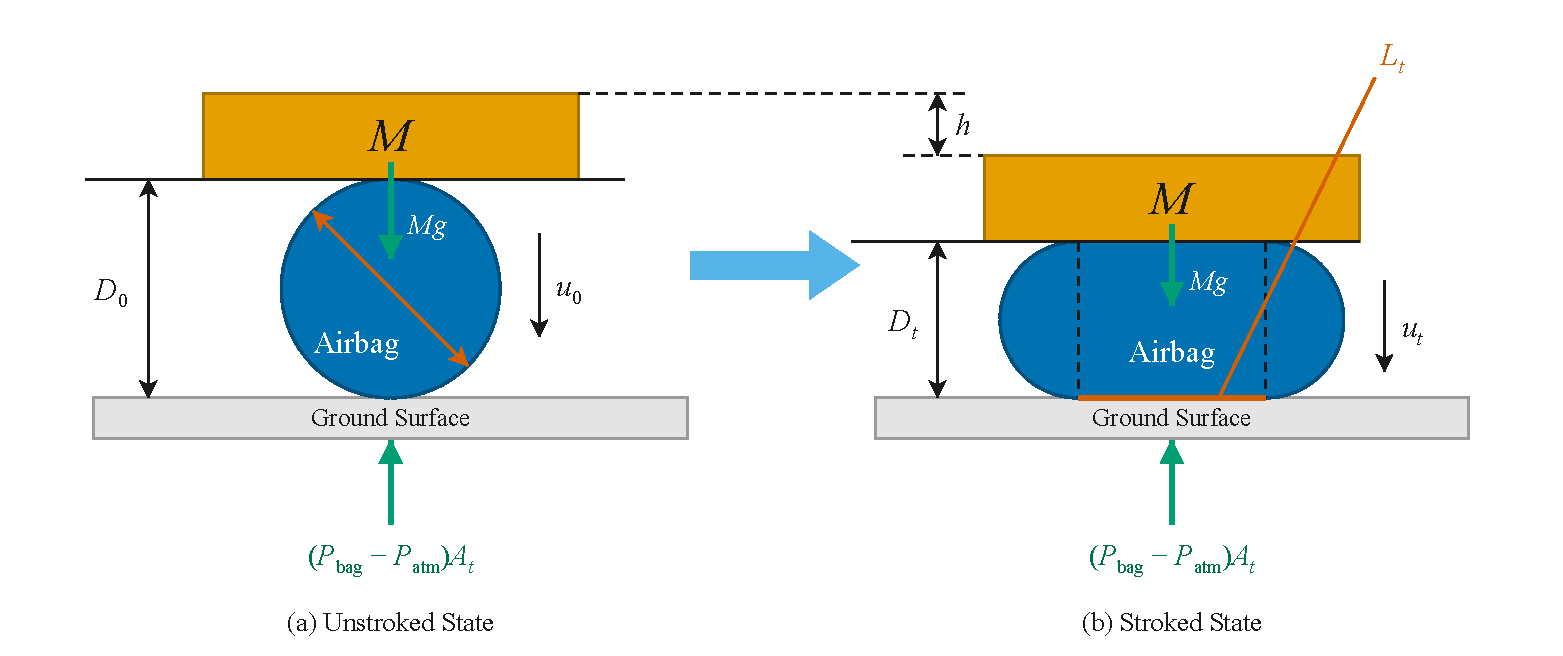
\includegraphics[width=\textwidth]{figures/chap2/Zhou-et-al_2019_diagram.pdf}
    \caption{One-degree-of-freedom airbag impact model in the unstroked (a) and stroked (b) states, adapted from Zhou et al. \cite{Zhou2019}.}
    \label{fig:zhou-airbag-1dof}
\end{figure}


The quantities under study for this type of phenomenon are shown in Fig.\ref{fig:zhou-airbag-1dof}, where a point load (yet, with a finite extension, as to avoid penetration in the airbag and justify the crude, though analytically necessary, \textit{uniform pressure/control volume} assumption, where pressure is uniformly distributed within the airbag volume) is protected by a single inflated airbag in incipient contact with the ground surface after a free fall. The quantities are:

\begin{itemize}
  \item $M$, the mass of the payload, which remains constant throughout the analysis and results in the vertically applied gravitational force $M g$.
  \item $u_0$, the initial impact velocity at time $t_0$, which evolves to $u_t$ after each subsequent time increment. It is updated at every time increment through kinematic analysis.
  \item $D_0$, the initial diameter of the airbag, which evolves to $D_t$ following the same loop update concept. Broadly speaking, its meaning can be extended to the characteristic dimension of the airbag, according to the airbag shape selected for the test case among the available options (vertically- or horizontally-oriented cylinder, sphere, toroid, etc.).
  \item $h$, the \textit{stroke}, i.e. the (vertical) distance covered by the payload when compressing the airbag during the impact event.
  \item $(P_{bag}-P_{atm})\cdot A_t$, the normal reaction force from the ground, based on the difference between the internal pressure of the airbag $P_{bag}$ and atmospheric pressure $P_{atm}$, multiplied by the footprint area $A_t$ with the ground, calculated according to different geometric assumptions correlating $A_t = f(h,t)$.

\end{itemize}

The reference system is downward-positive, in accordance with the direction of gravity and the initial velocity, making the reaction force negative.

\begin{figure}[h]
    \centering
    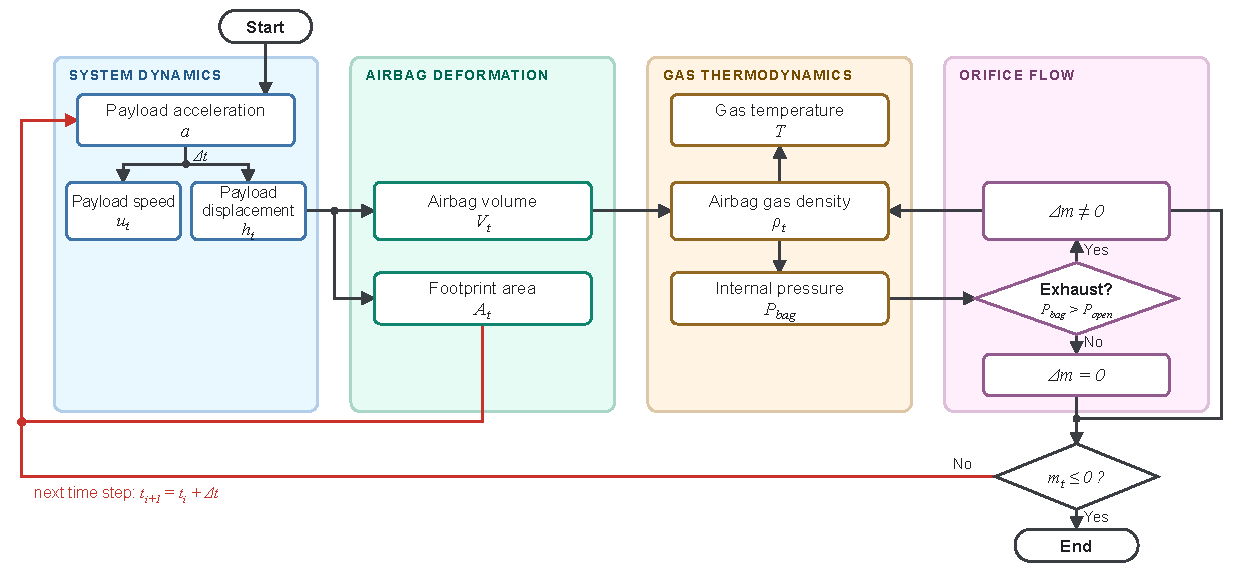
\includegraphics[width=\textwidth]{figures/chap2/Zhou-et-al_2019_flowChart.pdf}
    \caption{\hl{manca per caso la freccia di terminazione?} Calculation flowchart of the one-degree-of-freedom airbag impact model, adapted from Zhou et al. \cite{Zhou2019}.}
    \label{fig:zhou-airbag-flowchart}
\end{figure}

Except for the initial conditions and the payload's mass, these quantities are updated iteratively at each timestep to produce characteristic outputs for airbag-governed impact events such as \textit{airbag volume}, \textit{internal pressure}, \textit{internal gas mass}, \textit{payload acceleration}, \textit{payload speed}, and \textit{payload displacement}. The logic of this calculation loop is schematized in Fig.\ref{fig:zhou-airbag-flowchart}, which is an adaptation of the original diagram presented in the paper. The calculation loop is divided into four blocks, run sequentially at each timestep:

\begin{enumerate}
  \item \textbf{System dynamics step}: The resultant acceleration $a$ acting on the payload is calculated based on the reaction force from the ground calculated in the previous time step, and then integrated using the \textit{\hl{central difference scheme NEEDS MORE DETAIL?}} to obtain payload velocity $u_t$ and displacement (or stroke) $h$.
  \item \textbf{Airbag deformation step}: The airbag volume $V_t$ and footprint area $A_t$ on the ground surface are updated according to the kinematic information from the previous timestep. In this step, the hypothesis linking the stroke to the footprint area is enforced based on geometric assumptions, as mentioned earlier.
  \item \textbf{Gas thermodynamics step}: The state variables of the gas are updated assuming adiabatic compression, as it is safe to assume that little to no heat is exchanged during the rapid compression process.
  \item \textbf{Orifice flow step}: This critical step accounts for energy dissipation during the impact event. By modelling the outward airflow as flow through a one-way valve, treated as an orifice embedded in an impermeable fabric, typical nozzle fluid dynamics equations are applied to calculate the $\Delta m$ vented at each timestep. In the case of this specific paper, mass is vented only if the internal pressure $P_{bag}$ exceeds threshold pressure $P_{open}$, greater than atmospheric pressure $P_{amb}$. Within a single timestep, venting takes place as long as the exhaust condition withstands, updating gas density $\rho_t$ and recalculating the gas' temperature $T$ and pressure in an internal feedback loop. 
\end{enumerate}

In \cite{Zhou2019}'s framing, the code stops either when the manually-set duration of the phenomenon is reached, or when all mass is vented off. Testing of the code indicates that the no-rebound condition shown in the paper is numerically enforced by introducing an if-check managing the application of the reaction force.

The core work of the present thesis resides in turning the working principle of airbag impact events as presented in \cite{Zhou2019} into an informed, multi-variable problem that requires numerical optimisation. The code presented in later Section \ref{section:optimisation-code} is an expanded version of this implementation, incorporating additional criteria and alternative termination mechanisms.


\subsection{Design guidelines, requirements, and variables}\label{section:airbag-design-guidelines}
\subsubsection{Framing}
In essence, an airbag can be considered as an energy absorber and dissipator that must bring the payload from its impact velocity $v$ to rest within an available stroke $h$, without exceeding an allowable deceleration $a$. This relation is expressed in its most basic form by the kinematic relation \cite{Smith2007,Crane1985}
\begin{equation}
    h = \frac{v^2}{2a}
    \label{eq:basic-stroke-calc}
\end{equation}
which shows the central trade-off in airbag design: the lower the allowable deceleration, the longer the stroke needed to decelerate the payload and, therefore, the larger the airbag. During compression, the airbag behaves as a non-linear spring whose stiffness depends on its geometry and venting characteristics \cite{DoDeWeck2012,Zhou2019,Cole1993}. Venting is what dissipates the absorbed energy \cite{DoDeWeck2012}; whatever energy remains stored in the gas at the end of the stroke is returned to the payload as rebound \cite{WarrickLee2001}. Increasing the volume of the airbag and inflation pressure raises its energy dissipation capacity, but at the cost of higher membrane loads on the fabric \cite{Smith2007,DoDeWeck2012}.

\subsubsection{Configuration concepts}
Airbags are generally classified into three types depending on whether they contemplate the presence of venting in their design: \textit{non-vented}, \textit{vented}, and \textit{combined} \cite{Zhou2019}. A combined airbag usually consists of an outer, main-venting airbag and an inner, non-venting, anti-bottoming airbag. This "bag within a bag" concept prevents the payload from bottoming out once the outer bag has vented \cite{DoDeWeck2012,Tutt2008,GardinierTaylor1999}, and commonly relies on complex sequential inflation of the outer and inner bags \cite{GardinierTaylor1999}. An alternative to this design is using multiple airbags side by side rather than one within the other, following a "fail-safe" design philosophy by sharing impact loads and providing redundancy in case of airbag failure \cite{Smith2007}. Rather than completely enveloping the payload, the airbag can act as a buffer cushion beneath it \cite{GardinierTaylor1999}, or inflate between plates attached to the sides of the cargo \cite{Taylor2001}. Moreover, venting can be passive, activated pneumatically, or active, activated electronically \cite{WarrickLee2001,HolnickiSzulc2009}. Active venting is the basis of adaptive impact absorption, in which the airbag responds to the actual, case-specific impact load \cite{HolnickiSzulc2023}: for example, in multi-chamber designs, controllable valves allow gas to flow between adjacent chambers and to the environment, redistributing a non-uniform load across the structure \cite{HolnickiSzulc2009,HolnickiSzulc2015}.

\subsubsection{Design requirements}
Notable airbag design requirements and recommendations identified in literature are summarised in Table \ref{tab:requirements} and relate to impact conditions, such as the vertical and horizontal velocity, impact attitude, and landing surface \cite{McCullough1964,Smith2007,DoDeWeck2012}; to the allowable deceleration of the payload; and to general constraints on mass, packaging volume and deployment time \cite{HolnickiSzulc2023,GardinierTaylor1999,Cadogan2002}.

% requirements table
{\longtablesetup
\begin{longtable}{G{0.19} L{0.51} L{0.30}}
\caption{Design requirements for airbag landing and impact-attenuation systems identified in the literature.}
\label{tab:requirements}\\
\headrow\hd{Category} & \hd{Requirement} & \hd{Sources} \\
\endfirsthead
\headrow\hd{Category} & \hd{Requirement} & \hd{Sources} \\
\endhead
\contfoot{3}
\endfoot
\lastrule
\endlastfoot

% ---------------------------------------------------------------------
Dynamics
& Limit the peak acceleration transmitted to the payload & \cite{HolnickiSzulc2023,GardinierTaylor1999,Lim2015,DoDeWeck2012,Alekseychuk2024} \\
\itemrule{2}
& Reduce the touchdown velocity to a target value & \cite{HolnickiSzulc2023} \\
\itemrule{2}
& Cope with horizontal velocity (non-nominal impact attitudes coupling) & \cite{Smith2007,DoDeWeck2012,McCullough1964} \\
\grouprule
% ---------------------------------------------------------------------
Landing conditions
& Cope with different landing surfaces & \cite{McCullough1964,Shen2025,Tutt2008} \\
\itemrule{2}
& Avoid fabric rupture and tearing & \cite{DoDeWeck2012,Cadogan2002} \\
\itemrule{2}
& Prevent bottoming-out of the payload & \cite{GardinierTaylor1999,DoDeWeck2012,Tutt2008,Zhou2019} \\
\itemrule{2}
& Limit rebound and prevent rollover & \cite{WarrickLee2001,GardinierTaylor1999} \\
\grouprule
% ---------------------------------------------------------------------
Inflation pre-landing
& Synchronise venting and payload contact & \cite{CasidayFrey2000} \\
\itemrule{2}
& Deploy fully within the available time & \cite{HolnickiSzulc2023,GardinierTaylor1999} \\
\itemrule{2}
& Retain pressure for the required duration & \cite{GardinierTaylor1999,Cadogan2002} \\
\grouprule
% ---------------------------------------------------------------------
Packaging
& Survive long-term stowage in the packed state & \cite{Cadogan2002} \\
\itemrule{2}
& Integrate with the host vehicle without interference & \cite{HolnickiSzulc2023} \\
\itemrule{2}
& Withstand the environmental temperature range & \cite{Cadogan2002,McCullough1964} \\
\grouprule
% ---------------------------------------------------------------------
General
& Minimise system mass & \cite{HolnickiSzulc2023,GardinierTaylor1999,Cadogan2002} \\
\itemrule{2}
& Allow reuse & \cite{GardinierTaylor1999,McCullough1964} \\
\itemrule{2}
& Provide redundancy against single-bag failure & \cite{Smith2007} \\
\end{longtable}
}


\subsubsection{Design variables}
All airbag design variables found in the literature analysed for the present review can be found in Table \ref{tab:variable_inventory}. The variables in the table are divided into two umbrella categories: \textit{Energy absorption at impact} and \textit{Deployment and packaging}. These categories can be mapped almost directly onto two distinct impact phases (at-impact and pre-impact behaviour, respectively) and, consequently, into two separate, although not entirely uncoupled, design stages: \textit{phase 1}, focusing on the inflated configuration during impact to \textit{limit peak acceleration} below the allowable limit set by the payload's integrity requirement, and \textit{Phase 2}, focusing on the pre-impact inflation process by mostly \textit{optimising out-of-stowage deployment time} and leading to prototyping.

% mega long table
{\longtablesetup
\begin{longtable}{G{0.13} L{0.17} L{0.46} L{0.24}}
\caption{Airbag design variables identified in the literature, grouped by design focus and subcategory, with the associated trade-offs.}
\label{tab:variable_inventory}\\
\headrow\hd{Group} & \hd{Variable} & \hd{Trade-off} & \hd{Sources} \\
\endfirsthead
\headrow\hd{Group} & \hd{Variable} & \hd{Trade-off} & \hd{Sources} \\
\endhead
\contfoot{4}
\endfoot
\lastrule
\endlastfoot

% ---------------- GROUP 1 (blue = Phase 1)
\grouphead{4}{phaseA}{Energy absorption at impact}
Geometry
  & Shape & Pressure-vessel shapes carry membrane loads well; faceted shapes are easier to build & \cite{Zhou2019,Smith2007,Tutt2008,TaylorGardinier1999,DoDeWeck2012,Shen2025} \\
\itemrule{3}
& Characteristic size & More volume absorbs more energy but raises membrane loads, chance of rebound, and overall structural weight & \cite{Smith2007,DoDeWeck2012,WarrickLee2001,Peng2021} \\
\itemrule{3}
& Payload contact area & Larger contact spreads the load; wrapping the entire payload wastes material and increases weight & \cite{Tutt2008,GardinierTaylor1999,TaylorGardinier1999} \\
\itemrule{3}
& Number of chambers & Inner anti-bottoming and multiple bags add margin and redundancy (fail-safe philosophy), but increase weight and complexity & \cite{Zhou2019,DoDeWeck2012,Tutt2008,GardinierTaylor1999,Smith2007,HolnickiSzulc2009} \\
\itemrule{3}
& Tethers and webbing & Divert inertial loads from the fabric and control the shape, at the cost of added parts & \cite{Shen2025,Tutt2008,Tutt2009} \\
\grouprule
Fabric
  & Fabric type & Strength, tear resistance, low permeability, temperature flexibility vs.\ mass, packability & \cite{Cadogan2002,Tutt2008,Tutt2009,GardinierTaylor1999,Shen2025,Verma2025,Alekseychuk2024,CasidayFrey2000,Hirth2007,Lee2009,Dobrich2014} \\
\itemrule{3}
& Fabric thickness & Thicker fabric raises the rupture margin but slows deployment, enlarges the package, and increases weight & \cite{Yang2015,Lim2015,DoDeWeck2012} \\
\grouprule
Venting
  & Vent area & Larger orifices dissipate more energy and limit rebound, but risk bottoming-out & \cite{Smith2007,DoDeWeck2012,Cole1993} \\
\itemrule{3}
& Vent location & Sets the outflow and whether the ground or payload blocks the vent during the stroke & \cite{Tutt2008} \\
\itemrule{3}
& Vent burst pressure & Early opening lowers the peak pressure and resultant acceleration but spends stroke; late opening raises the peak pressure and acceleration & \cite{Smith2007,CasidayFrey2000} \\
\itemrule{3}
& Fabric porosity & Distributed gas leakage dissipates energy without vents but reduces pressure retention & \cite{Yang2015,Lim2015,KhanMoatamedi2008,Fokin2003,Cadogan2002} \\
\itemrule{3}
& Vent actuation & Active valves adapt to the actual impact; passive valves need no sensing or power & \cite{WarrickLee2001,HolnickiSzulc2009,HolnickiSzulc2015,HolnickiSzulc2023,Tutt2008,GardinierTaylor1999} \\
\grouprule
Gas
  & Initial bag pressure & Higher pressure stops the payload in a shorter stroke but raises membrane loads & \cite{Smith2007,DoDeWeck2012,CasidayFrey2000} \\
\itemrule{3}
& Gas composition & Specific-heat ratio sets compression stiffness; mixtures cut temperature sensitivity & \cite{CasidayFrey2000,Jang2021,Alekseychuk2024,Verma2025,Tutt2008} \\
% ---------------- GROUP 2 (teal = Phase 2)
\grouphead{4}{phaseB}{Deployment and packaging}
\tintB Inflation
  & Inflator type & Pyrotechnic vs.\ stored compressed gas: drives gas output, package size and triggering mechanism & \cite{Verma2025,Madlung1996,CasidayFrey2000,Jang2021,Tutt2008} \\
\itemruleB{3}
\tintB & Inflator supply pressure & Faster filling vs.\ higher deployment loads; the flow chokes at sonic conditions & \cite{KhanMoatamedi2008,CasidayFrey2000} \\
\itemruleB{3}
\tintB & Inflator mass flow rate & Shorter injection time vs.\ higher deployment loads & \cite{Yang2015,Lim2015,KhanMoatamedi2008} \\
\itemruleB{3}
\tintB & Inflator gas temperature & More pressure per unit gas mass vs.\ thermal load on the fabric just after inflation & \cite{Yang2015,Lim2015,Tutt2008,Cadogan2002} \\
\groupruleB
\tintB Housing
  & Housing size and geometry & Compact housings save mass and volume but pack the bag tighter & \cite{Munoz2007,Lim2015} \\
\itemruleB{3}
\tintB & Housing material & Plastic saves mass over metal; metal bases give a stiff mounting & \cite{Crane1985,Munoz2007,Verma2025,Lim2015} \\
\groupruleB
\tintB Folding
  & Folding pattern & Governs unfolding kinematics, deployment time and pre-stress in the packed fabric & \cite{Lee2009,Munoz2007,Ruff2007,Kamiji1998,Yang2015,Ritmeijer2005,KhanMoatamedi2008,Thornton2004,Cadogan2002} \\
\itemruleB{3}
\tintB & Number of folds & Smaller package vs.\ longer, less predictable unfolding & \hl{RIVEDI LIBRI DI MATEMATICA DELLA CERAGIOLI} \\
\groupruleB
\tintB Seams
  & Seam locations & Seams concentrate stress and are the main failure site; patterning minimises their number & \cite{Cadogan2002,Tutt2009,Bulathsinghala2021} \\
\end{longtable}
}

The table conveys the complexity of the design problem at hand, highlighting the large number of design variables. Multi-variable problems typically require an optimisation process where an optimal combination of variable values is achieved through guided iterations based on penalty concepts. This consideration forms the basis for the following chapters, in which the airbag design process is distilled into an ad-hoc workflow tailored for a specific payload application and impact scenario, focusing on a single design phase among the two presented. It is now possible to define the research-development objectives of the present thesis, leading to the proposed solution in Chapter \ref{chapter:methodology} and the specific implementation choices presented in Chapter \ref{chapter:results}.


\section{Research-Development Objective}

Having presented the context in which the research project is allocated and having gathered the necessary design information, it is possible to address the requirements set by the project commissioners:
\begin{itemize}
    \item Identify and characterise the mechanical allowables of typical medical payloads based on general packaging requirements for UAV-transported medical goods;
    \item Develop an informed conceptual design of an airbag system capable of deploying during emergency release conditions to absorb impact energy and preserve payload integrity.
\end{itemize}

These requirements can be summarised in the following Research-Development Objective and Research Questions:

\begin{objectivebox}{Research-Development Objective}
Develop and validate a design workflow to model and simulate an airbag-based protective system for UAV medical payloads using LS-DYNA, with the primary objective to ensure the structural integrity of pharmaceutical materials and their containment during drone failure and emergency payload release, thereby preventing environmental dispersion and supporting certification requirements.
\end{objectivebox}

\begin{objectivebox}{Research Question(s)}
How can a systematic multi-phase simulation workflow be developed to design an airbag-based protective system for medical payloads during UAV emergency-release events?

\textbf{Sub-questions:}
\begin{enumerate}
    \item What are the allowable mechanical limits (acceleration, stress, etc.) for medical products during emergency release, and how should these define the design envelope?
    \item How can the inflated airbag configuration be optimised to satisfy impact-absorption requirements while balancing competing design requirements?
    \item What recommendations facilitate transforming the inflated geometry into a compact, functional deployment system?
\end{enumerate}
\end{objectivebox}

% LTeX: language=en-GB
\chapter{Methodology: the Airbag Design Workflow}
\label{chapter:methodology}


\section{Problem statement}
To properly outline and, more importantly, test the workflow proposed as a main objective of this thesis, it is necessary to identify the specific context in which this project is embedded, as it originates from prior research work conducted within the specific framework of Turin. The design inputs presented below were gathered from analysing the results presented by the group (\cite{Cavallo2020}, \cite{Bertelli2021}, \cite{Sivieri2021}, \cite{Fiorentino2021}, and \cite{Angelini2023}) and categorising them into mission aspects on which to root the proposal of Section \ref{section:proposed-approach}.

\subsection{Reference mission and design inputs}
\subsubsection{Route and flight profile}
The reference mission is based on a hospital-to-hospital route as initially suggested by Cavallo (2020) \cite{Cavallo2020}, connecting two hospitals across the city of Turin as shown in Fig. \ref{fig:trajectory-map}, representing a city map with route schematics. In particular, the starting point is the Molinette Hospital in the southern region of the city, and the destination is the San Giovanni Bosco hospital in the northern sector. As they are located far apart, these two hospitals require medical deliveries to traverse a broad part of the city's territory. The hospitals are connected through two possible routes:
\begin{itemize}
    \item \textbf{Route A}: Initially hypothesised by Cavallo and confirmed by Bertelli (2021) \cite{Bertelli2021}, it takes advantage of the above-water air corridor over the river Po and its tributary Stura, mostly skirting the city and flying over city ground only in the relatively short segments connecting the hospitals to the rivers. Among the two routes, it is the safest (and, thus, most certifiable according to Cavallo) as it reduces the probability of ground impact in case of drone failure due to the UAV's permanence in the above-water air corridor. This route was selected as viable within the Concept of Operations (ConOps) that informed the preliminary drafting of the SORA. Approximate length: 10\,km. Approximate duration time: 15\,min, comparable to ambulance-based delivery times.
    \item \textbf{Route B}: A crude alternative to Cavallo and Bertelli's Route A, connecting the two hospitals in a straight line over the city. Angelini (2023) \cite{Angelini2023} deemed this route infeasible based on their comparative safety analysis of delivery means, primarily due to the lack of proper risk mitigation measures concerning in-flight failures. However, as the approach proposed in this thesis aims at partially mitigating these risks, it was chosen to consider this route (at least for preliminary evaluation).
    \item \textbf{Alternative routes \textit{(omitted from analysis)}}: Fiorentino (2021) \cite{Fiorentino2021} and Angelini (2024)'s \cite{Angelini2023} work is rooted in minimum risk-based route selection considering territories that extend beyond city borders, specifically including the entire province\footnote{In Italy, local government is organised across three administrative levels: regions, provinces, and municipalities. Here, assessing the Province of Turin corresponds to evaluating the territorial sub-region of Piedmont administered by the provincial capital of Turin.} in case of Angelini's study. Either using the RRT* algorithm in Fiorentino's case or the Dijkstra and A* algorithms in Angelini's case, these two studies share a common approach of considering multiple layers (\hl{such as population density, shelters, and critical infrastructure CHECK}) to calculate the probabilistic minimum-risk paths for different means of transportation (eVTOL, UAV, etc.), without predefined start and end points, thereby determining the optimal drone hub location across the province. \hl{valid for FIORENTINO TOO???} The results of these works were omitted from the definition of the reference mission for two main reasons. First, they do not specifically target hospital-to-hospital operations; their scope focuses on optimising general logistics rather than facilitating inter-hospital transport, contrarily to one of the primary objectives of the present thesis. Second, their findings indicate that drone operations, when evaluated against the merit indices adopted in their analyses, are deemed unviable due to safety constraints. In contrast, the objective of this research is precisely to identify a mission scenario that is unfeasible under current conditions and implement risk-mitigation strategies to ultimately enable drone transit.
\end{itemize}


In either Route A or B, as specified in Bertelli's ConOps, the cruising height is about 75\,m, at 17\,m/s cruising velocity (approximately 70\% of the maximum cruising speed allowed by the UAV platform of 25\,m/s, unsustainable for the entire duration of the mission at the time of evaluation), with possible speed variations according to mission urgency if specified in the ConOps. 

Accounting for the presence of wind in the operating environment, wind speed in Turin averages about 1.8\,m/s (6.5\,km/h) \cite{ComuneTorinoWind-AVG}, with a peak of about 28.6\,m/s (103\,km/h) in 2013 \cite{ComuneTorinoWind-MAX}.

\begin{figure}[h!]
    \centering
    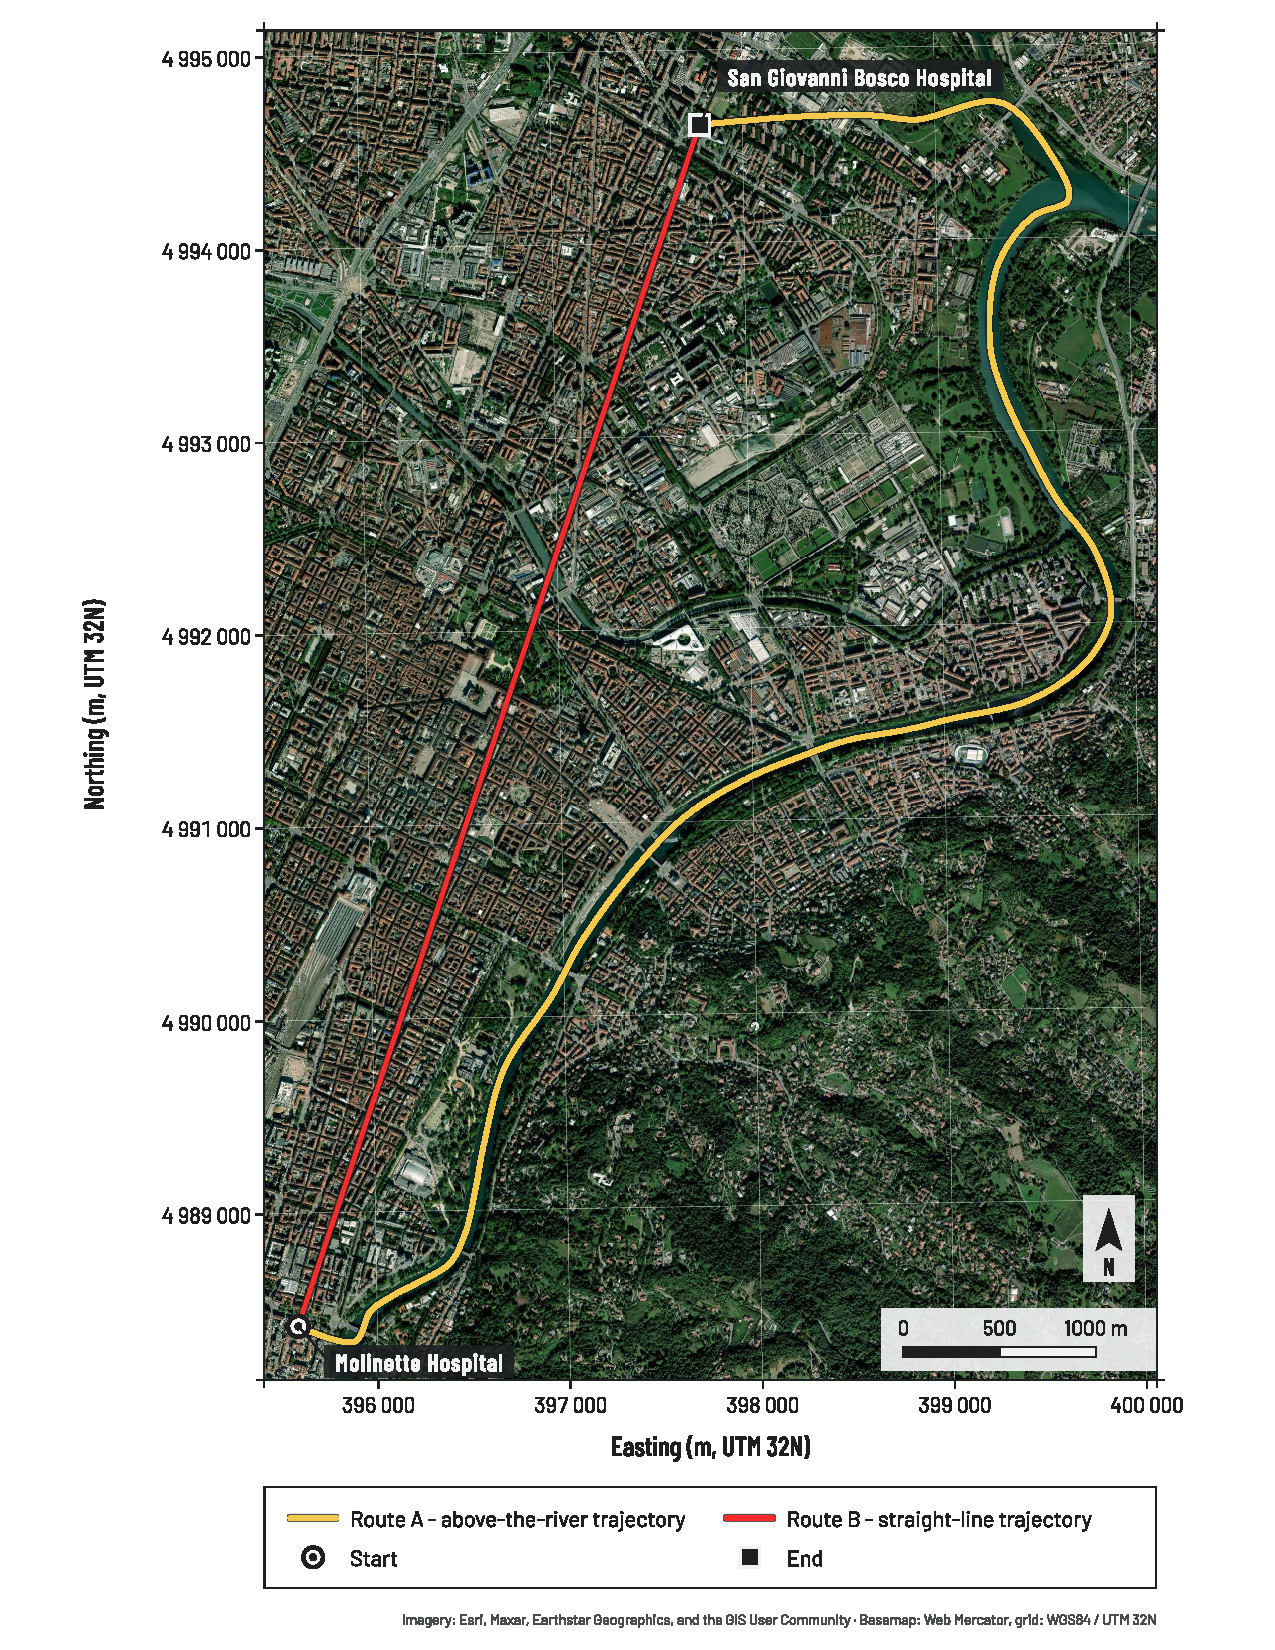
\includegraphics[height=0.54\textheight, keepaspectratio, trim=35 24 41 7, clip]{figures/chap3/trajectory-map-satellite.pdf}
    \caption[Reference mission routes across Turin]{Reference mission routes across Turin, from the Molinette Hospital to the San Giovanni Bosco Hospital: Route A (above-the-river trajectory) and Route B (straight-line trajectory).\protect\footnotemark}
    \label{fig:trajectory-map}
\end{figure}
\footnotetext{Imagery: Esri, Maxar, Earthstar Geographics, and the GIS User Community. Basemap: Web Mercator; grid: WGS84 / UTM 32N.}


\subsubsection{UAV Platform}
The UAV platform choice is inherently linked to the reference mission specifications above, meaning that the platform is required to sustain the cruising speed requirements specified in the ConOps. A Maximum Takeoff Mass (MTOM) of 9\,kg and a 0.81\,m characteristic dimension were also specified in Bertelli's ConOps, leading to the suggestion of a potential drone model suitable for the situation: DJI's \textit{Matrice 300 RTK}. Despite having characteristics suitable for the speed requirements, the drone has a payload limit of 2.7\,kg and a wind resistance of 15\,m/s in cruise. While this drone was initially selected for the preliminary SORA, its specific parameters are not binding for the present study. In particular, the payload-mass and wind-resistance limitations may be disregarded, given that the ConOps set a much broader requirement for MTOM. In addition to these requirements, Cavallo, in their UAV platform market evaluation, considered several other factors: maximum flight time (usually corresponding to half the autonomy), geometry, glide speed, and frontal area, the latter covering an important role in free-fall drag calculations. By ConOps, the platform is equipped with a parachute, whose contribution is ignored in the calculations regarding the free-fall event. 

\subsubsection{Failure scenario and impact conditions}
The chosen failure scenario implies an in-flight malfunction or fatal failure of the UAV in combination with a failure of the parachute mounted on the drone by ConOps. Excluding the nominal, non-conservative parachute descent of 3\,m/s estimated by Bertelli, in this extreme failure scenario the payload is dropped in free air, separated from the drone at an altitude of 75\,m above ground. After the failure, a \textit{ballistic} descent mode is chosen for calculations of impact time and point depending on the release position on the map, including the effects of gravity and aerodynamic drag (as opposed to \textit{uncontrolled glide} descent mode, which is applicable to the UAV platform but not to its detached payload), used in Angelini's impact probability study for ground risk evaluation and inspired by \hl{PRIMATESTA' CHECK!!!}. Wind enters the calculations (as mentioned in the reference route definition) as a horizontal velocity component.


\subsubsection{Payload container}
The design of the payload container to be carried by the UAV platform in delivery missions was proposed, but never fully prototyped, by Sivieri (2021) \cite{Sivieri2021}. Its geometry is shown in Fig. \ref{fig:payload_container} as modelled for the scope of the present thesis: the central body is a cylinder capped with two hemispherical domes. In Sivieri's original design, this container had to be constructed via stratifying four layers, from inside out: first layer of 3d-printed PET-G with thickness 2\,mm, second layer of manually applied thermal insulation of unknown effective thickness, third layer of 3D-printed PET-G and 2\,mm thickness, and a final layer of manually-applied thermo-reflective paint. This sandwich-type structure was designed specifically for evaluating the thermal and vibration loads of a reference mission similar to the one presented earlier, and thus avoiding making considerations on transportability, attachment mechanisms, and other application-specific parameters. From a structural perspective, the first and third layer of Sivieri's design were connected by four radial ribs, but this detail was deliberately omitted in the exemplification of the payload container for modelling simplicity and redundancy, as explained later in Section \ref{section:step4-sledTest}. 

\begin{figure}[h!]
    \centering
    \begin{subfigure}[b]{0.3\textwidth}
        \centering
        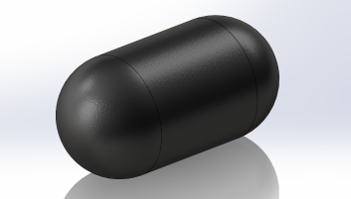
\includegraphics[width=\textwidth]{figures/chap3/payload_container_full.png}
        \caption{Full view of the closed container.}
        \label{fig:payload_container_full}
    \end{subfigure}
    \begin{subfigure}[b]{0.3\textwidth}
        \centering
        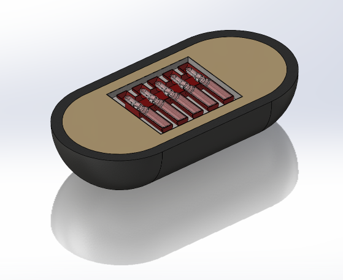
\includegraphics[width=\textwidth]{figures/chap3/payload_container_section.png}
        \caption{Sectioned view showing the outer shell, the foam filling, and the housed payload.}
        \label{fig:payload_container_section}
    \end{subfigure}
    \caption[Payload container geometry]{\hl{IT's REALLY UGLY}Payload container geometry: cylindrical central body capped with two hemispherical domes.}
    \label{fig:payload_container}
\end{figure}

Due to the artisanal nature of this design, linked to the difficulty in modelling specific 3D-printed PETG and the unquantifiable specifications of the insulation material, the payload container was modelled by retaining its shape with a 5 mm thick shell [\hl{verify thickness in the FE model}] of injection-moulded Acrylonitrile butadiene styrene (ABS), commonly used in packaging. The cavity is filled with polyurethane foam, chosen to simulate a protective wrapping (such as bubble wrap) that medical operators would use as established praxis to mitigate vibrations. The thermal paint is omitted from the payload container modelling process.



\subsubsection{Payload}
Considering the wide variety of medical goods potentially suitable for UAV-based air transport, it was necessary to identify a payload representative of standard shipments, excluding human organs and specialized equipment (e.g. defibrillators) to focus specifically on pharmaceuticals. Therefore, glass phials of the medicinal product \textit{Akineton Fiale}, containing \textit{biperidene lactate} at a concentration of 5\,mg/ml in injectable solution and shown in Fig.\ref{fig:akineton}\footnote{Source of photo: \url{https://www.guttafarm.net/akineton-cena}.}, were chosen. The product is commercially supplied in boxes of five phials, each individually packaged in a plastic blister tray.

\begin{figure}[h!]
    \centering
    \begin{subfigure}[b]{0.25\textwidth}
        \centering
        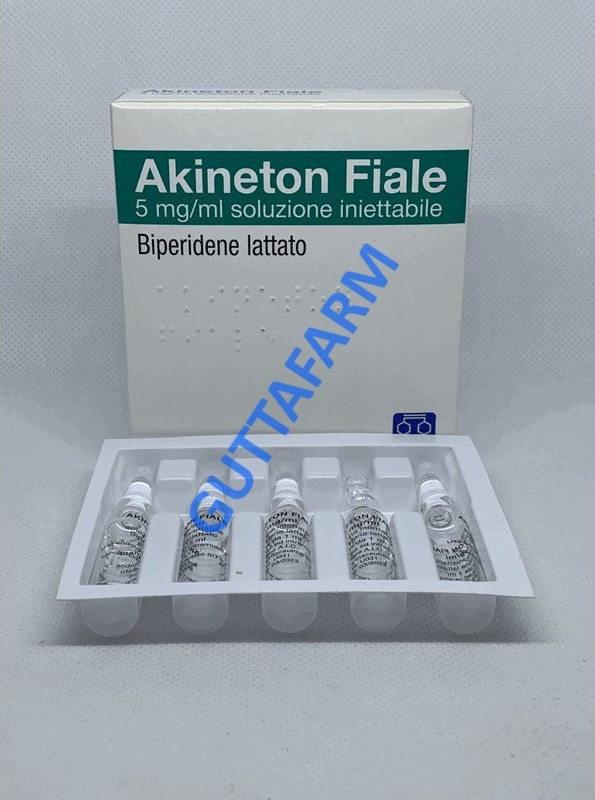
\includegraphics[width=\textwidth]{figures/chap3/akineton_fiale.jpg}
        \caption{Akineton Fiale, 5\,mg/ml injectable solution, as supplied in its original packaging.}
        \label{fig:akineton_box}
    \end{subfigure}
    \begin{subfigure}[b]{0.37\textwidth}
        \centering
        \includegraphics[width=\textwidth]{example-image-b}
        \caption{\hl{Single Akineton phial.}}
        \label{fig:akineton_phial}
    \end{subfigure}
    \caption{Akineton Fiale packaging and single phial.}
    \label{fig:akineton}
\end{figure}

Akineton is a pharmaceutical product commonly used in the treatment of Parkinson's disease and drug-induced extrapyramidal symptoms, and is usually administered by intravenous or intramuscular injection. For the purposes of the present thesis, only the mechanical properties of the glass container are of interest, as the pharmacological action of the medical fluid is not relevant to the type of structural analyses implemented in this study.


\subsection{Information gap}
The only missing inputs required for a full design workflow evaluation are:
\begin{itemize}
    \item The derived \textit{impact velocity}, angle, and mass for the selected scenario;
    \item The quantification of the phials' fragility through the characterisation of their material's mechanical \textit{allowables};
\end{itemize}

These failure scenario data must be fed into the design loop(s) proposed below to enable an effective design of the airbag-based impact attenuation system.

\section{Proposed approach}\label{section:proposed-approach}
\subsection{Outer design loop: formalising the \textit{Safety-First} principle}\label{section:outer-design-loop}

In response to the gap identified in Section \ref{section:payload-first-approach}, the first cotribution of this thesis is to propose an alternative design approach adopting (and later testing) the following guidelines:

\begin{objectivebox}[colframe=green!45!black, colback=green!60!black!8]{\textit{Safety-First} Design Principle}
\begin{enumerate}
\item The airframe and payload must be considered as two distinct entities;
\item In the type of operations considered, saving the payload takes higher priority than saving the airframe (carrying organs, expensive vaccines, emergency medicines, or high-value medical equipment is worth more than the drone itself);
\item Overall, the objectives are to minimise or mitigate:
    \begin{itemize}
    \item ground impact consequences,
    \item payload damage (preserving its integrity),
    \item environmental dispersion;
    \end{itemize}
\item These considerations should be applied at the beginning of the design process, possibly by integrating multiple safety devices (e.g., an airbag and a parachute working in tandem) and adjusting flight-mechanics considerations accordingly.
\end{enumerate}
\end{objectivebox}

A direct consequence of applying the Safety-First design principle in UAV-based operations' design is changing the sequence of design events, as exemplified in the simple flowcharts of Fig. \ref{fig:flowcharts-mission-vs-safety}, where Fig. \ref{fig:flowchart-mission-first} and Fig. \ref{fig:flowchart-safety-first} compare scenarios in which the mission loop can be interchanged with the safety loop to achieve design convergence. 


\begin{figure}[!htb]
    \centering
    \begin{subfigure}[t]{0.3\textwidth}
        \centering
        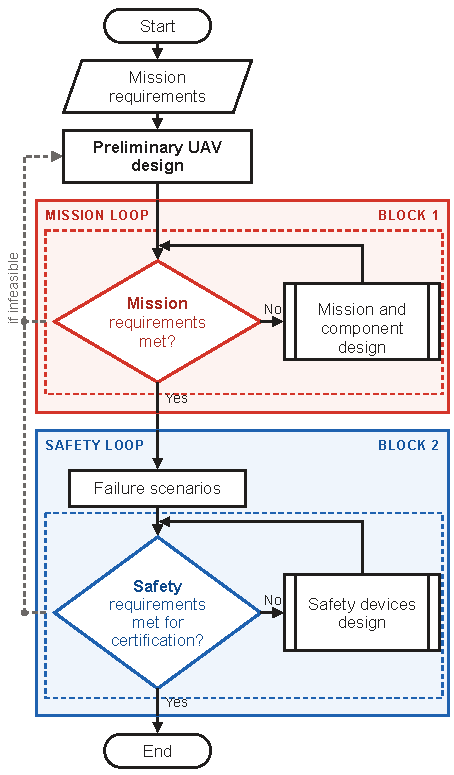
\includegraphics[width=\textwidth]{figures/chap3/flowchart-mission-first.pdf}
        \caption{\textit{Mission-First} approach}
        \label{fig:flowchart-mission-first}
    \end{subfigure}
    \hspace{0.08\textwidth}
    \begin{subfigure}[t]{0.3\textwidth}
        \centering
        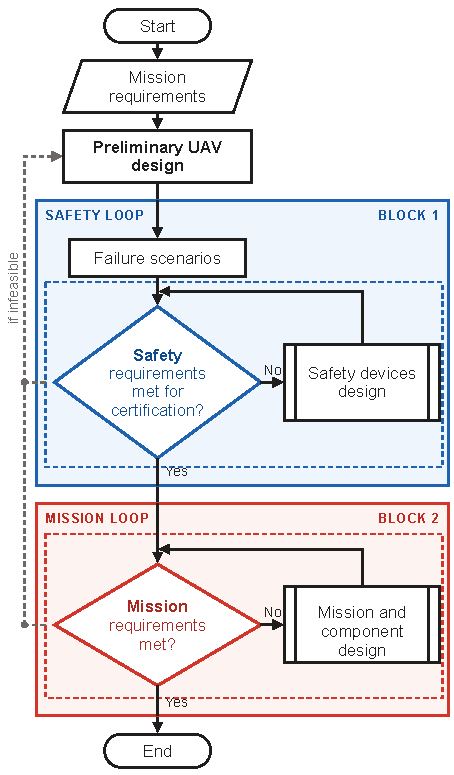
\includegraphics[width=\textwidth]{figures/chap3/flowchart-safety-first.pdf}
        \caption{\textit{Safety-First} approach}
        \label{fig:flowchart-safety-first}
    \end{subfigure}
    \caption{Sequence of design events in the two approaches: \textit{mission-first} and \textit{safety-first} loops.}
    \label{fig:flowcharts-mission-vs-safety}
\end{figure}



\subsection{Inner design loop: a payload-protection subsystem design workflow}\label{section:inner-design-loop}
This section aims to expand the \textit{Safety loop} concept presented in Section \ref{section:outer-design-loop} by informing it with the design guidelines distilled in Section \ref{section:airbag-design-guidelines}. The proposed workflow can be seen in Fig. \ref{fig:inner-design-loop}, and is divided into seven steps that bridge the gap between payload allowables' evaluation and safety device (airbag) prototyping. The loop is also split into two main branches, highlighting the boundary between the present MSc Thesis' deliverable and steps left to future developers. The first branch (steps 0-4) is partially payload-specific, meaning that some of the considerations made throughout these steps depend on the specific medical payload considered, while also generalisable to a broader spectrum of medical payload receptacles; the second branch (steps 5-7) are exclusively geometry-specific, implying that they require information on receptacle design, UAV-container hooking mechanism, and general information on system bulk, making them unattainable for the DIMEAS feasibility studies group, as they currently lack access to a functional medical payload container beyond their initial artisanal prototype by \cite{Sivieri2021}. Completing the workflow should lead directly to the \text{Mission loop} as shown earlier in Section \ref{section:outer-design-loop}.

\begin{figure}[!htb]
    \centering
    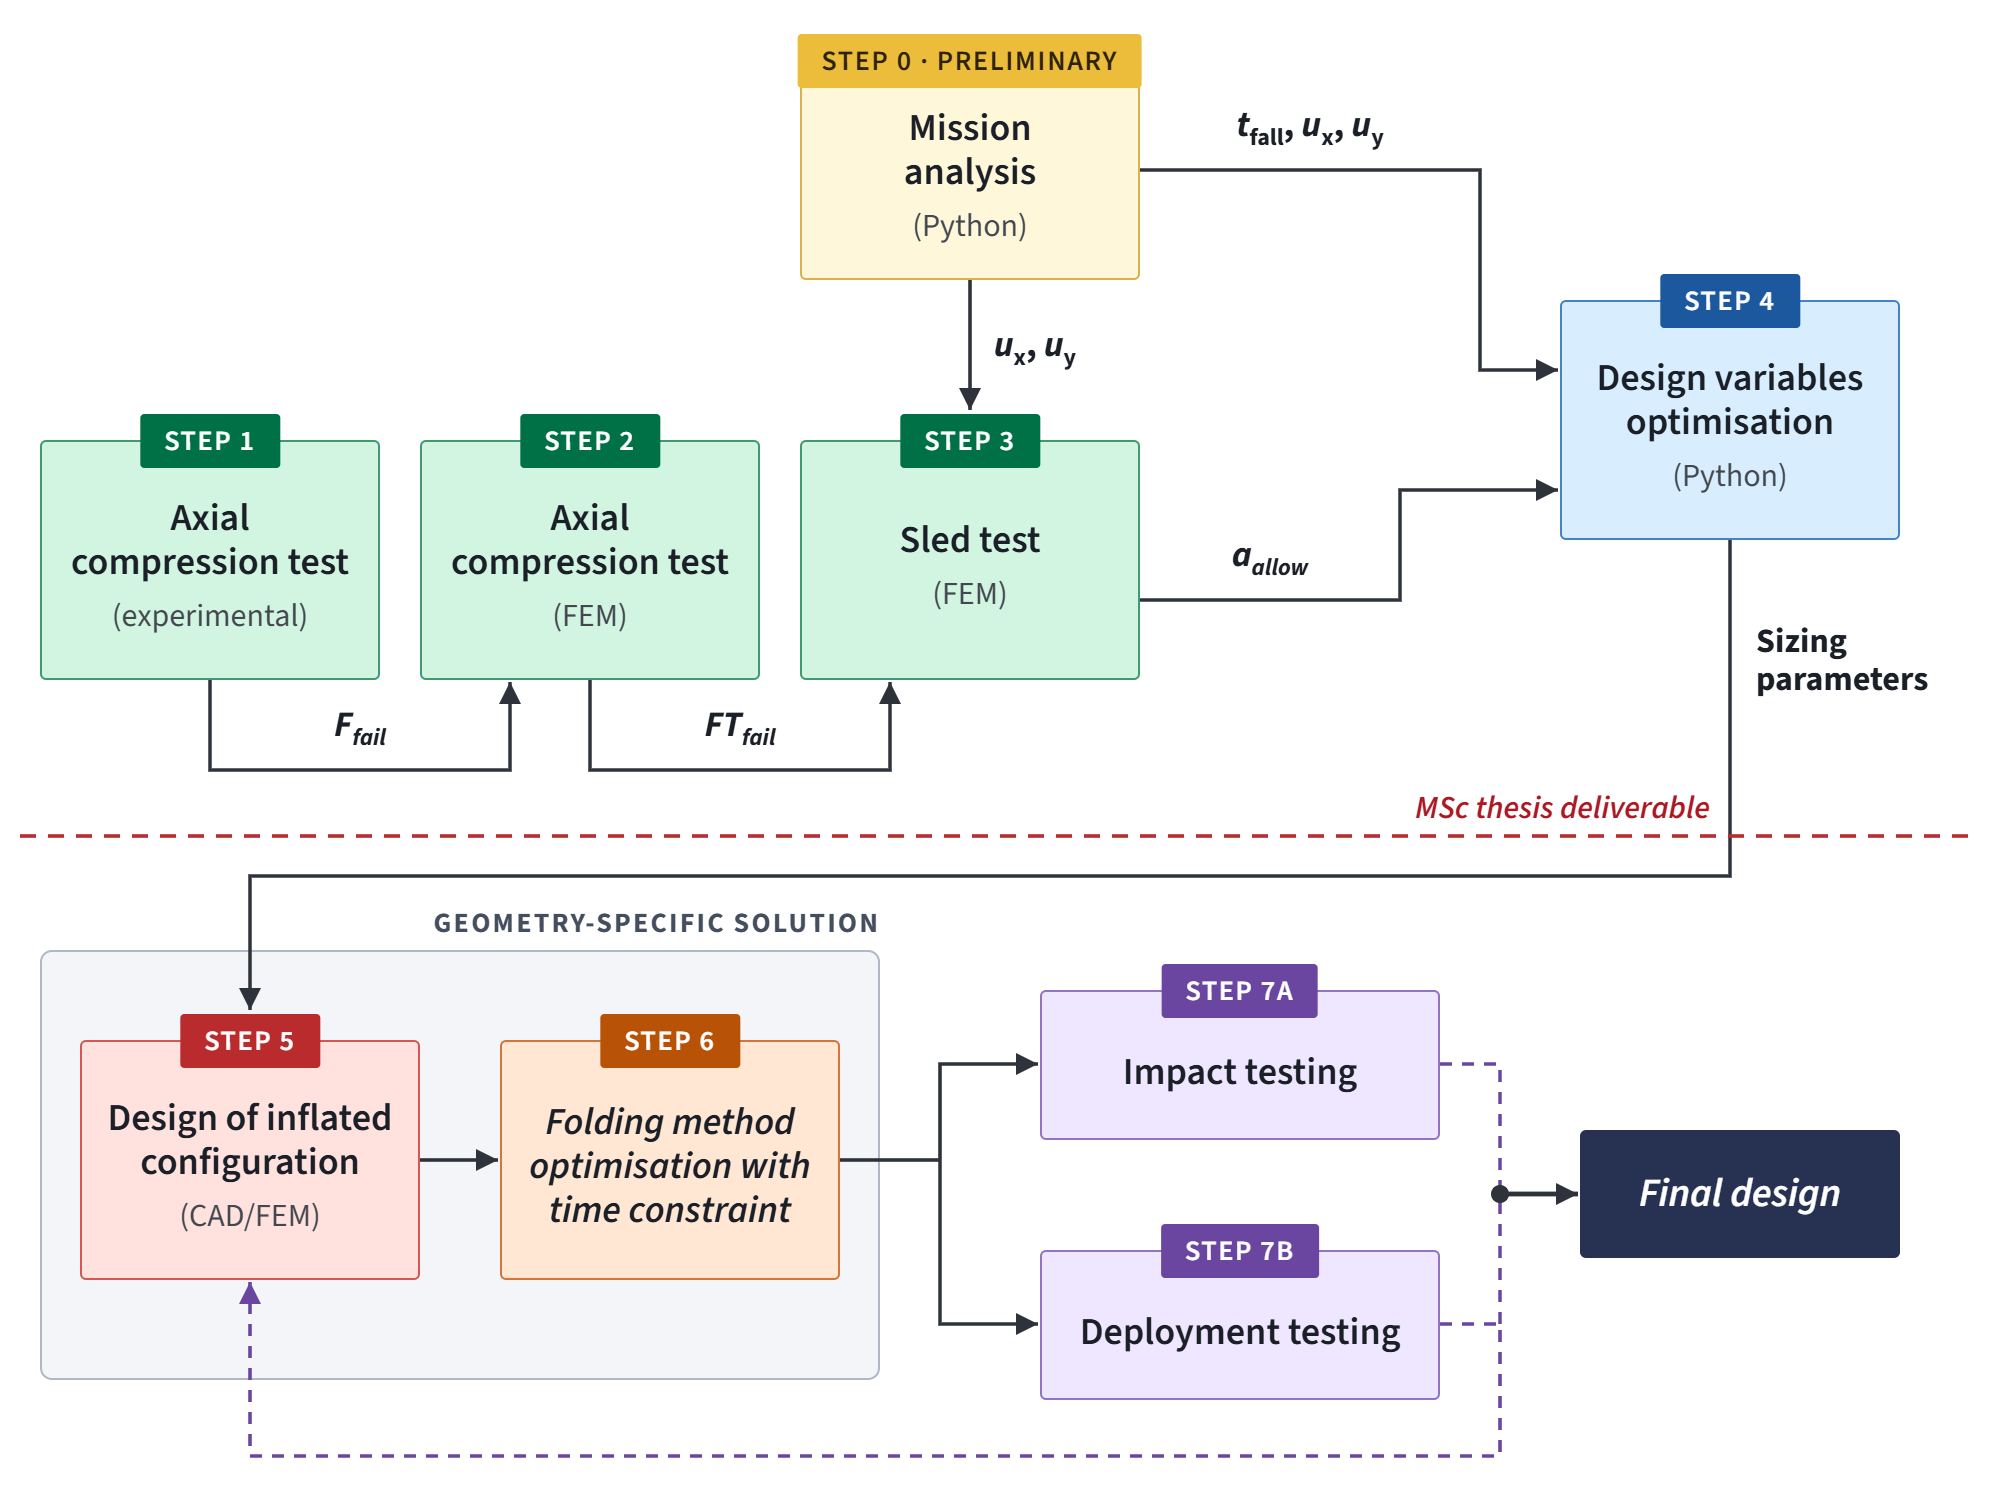
\includegraphics[width=0.85\textwidth]{figures/chap3/inner_loop_2-rows.png}
    \caption{Inner design loop, specific for the airbag-based payload-protection subsystem.}
    \label{fig:inner-design-loop}
\end{figure}


\subsubsection{Step 0 - Preliminary mission analysis}
This step covers the preliminary analysis of the payload's impact conditions. It evaluates the drop scenario, incorporates statistical analysis of wind direction and cruising conditions, and computes the trajectory and landing location of the payload. Serving as a general free-fall analysis, this phase yields key design inputs: the free-fall time ($t_{\text{fall}}$) and the horizontal and vertical impact velocities ($V_x$, $V_y$ respectively).

\subsubsection{Step 1 - Axial compression test (experimental)}
This step covers the experimental characterisation of the glass phials' (the selected medical payload) breaking point through laboratory testing. The goal is to conduct a test campaign to characterise the phial's mechanical behaviour, specifically providing key data, such as the failure force ($F_{\text{fail}}$, better defined in Section \ref{section:step1-test}), which feeds into the next phase to accurately calibrate the Finite Element Method (FEM) model.

\subsubsection{Step 2 - Axial compression test (FEM)}
This step focuses on matching the experimental behaviour observed in Step 1 with a Finite Element Method (FEM) model to accurately reproduce the material's mechanical response. Specifically, both experimentally and in the FEM model, the phials are subjected to axial compression loads, resembling the stress type to which they would be subjected to during an impact event. To replicate the laboratory results and build a calibrated material card that captures the phial's failure behaviour, the simulation mirrors the physical testing setup as closely as possible. This yields a generally realistic phial model, complete with its brittle failure threshold ($FT_{\text{fail}}$), that can be integrated into the full sled-test impact simulation in Step 3.

\subsubsection{Step 3 - Sled test}
This step involves simulating a sled test, heavily inspired by automotive industry practices, to observe the mechanical response of a test article (such as a dummy in vehicle crash testing, or in this case, a glass phial) measured through perceived accelerations and damage under an input acceleration profile. The simulated test subjects the payload container (based on the artisanal design proposed by \cite{Sivieri2021}) to realistic impact scenarios by reproducing an acceleration profile equivalent to a free-fall impact under the conditions defined in Step 0. This approach relies on the principle that the accelerations experienced by the payload directly correlate with the kinetic energy that must be dissipated during impact, linking the input acceleration profile to the resulting output. The primary output of this phase is the payload's allowable acceleration ($a_{\text{allow}}$).

\subsubsection{Step 4 - Design variables optimisation}
This fourth and final step of the thesis deliverable translates the established boundary conditions evaluated in previous steps (failure loads, allowable peak accelerations, impact velocities) into a numerical Python script for airbag sizing. Building upon the framework established in Section 2.1, the simulation optimises the airbag design against critical criteria, including total mass, bottoming-out speed, and rebound behaviour. Ultimately, this tool yields fundamental sizing parameters that will inform the future geometry-specific design of the system.


\subsubsection{Steps 5-7: Design of inflated configuration, folding method optimisation, impact and deployment testing}
Steps 5 and 6 shift the focus to geometry-specific development. Step 5 details the fully inflated configuration tailored directly to the geometry of the payload and UAV, matching the gas generator mechanism to the drone layout and impact timelines. Step 6 then builds upon this complete configuration by incorporating real-world manufacturing constraints, such as folding patterns, seaming details, and stowage volume, to optimise the deployment mechanism. While inherently interconnected, Step 6 specifically targets deployment time optimisation, as defined in Table \ref{tab:variable_inventory}.

Once a preliminary design and folding mechanism are established, the prototype undergoes a two-part experimental validation campaign: Step 7A (deployment testing) and Step 7B (impact testing). This phase validates the FEM models of steps 5 and 6 by subjecting physical prototypes to real-world impact conditions, operating in an iterative feedback loop between simulation and testing until design convergence is achieved.
 
% LTeX: language=en-GB
\chapter{Results: through the Workflow}
\label{chapter:results}

Do not include too many implementation details

\section{Mission and failure scenario analysis: calculating Vx and Vy}
* Mi servono degli input: prendo le informazioni raccolte nella fase preliminare di analisi missione (ref analisi missione)per stabilire probabilità di impatto and what not. 

* traiettoria
* punto di partenza, punto di arrivo
* drone scelto
* payload scelto
* medicinali scelti per simulazione

* serve energia di impatto?

---> risultati del WP2

\section{Studying the payload: calculating allowable impact acceleration}

\subsection{Material characterisation}
\subsubsection{TEST}
\subsubsection{FEM}
MENTION MODEL ITERATIONS TRIAL-AND-ERROR IN THE APPENDIX \ref{appendix:FEMiterations}!!!! FROM ABAQUS IMPLICIT TO CURRENT DECISIONS. Step by step, as in "version 1, abaqus implicit". Version 2, ls-dyna tetra elastic. Etc. MODAL PERTURBATION


* impact of container in LS-Dyna and what not. 
* diversi angoli di assetto per vedere il caso peggiore di accelerazioni locali
* cosa  possono sopportare le fialette e il contenitore????
* tipi di impatto, contenitore tipico che le contiene (menzionare la tesi del tipello) e che per il dimensionamento non viene considerato, approssimato a infinitamente rigido e che trasmette le accelerazioni di impatto così come le riceve ----> airbag deve essere dimensionato così
--------> tutte le analisi statistiche di prima, che hanno tenuto in considerazione anche il fatto che prima o poi si sorvolerà la città una volta risolti i cavilli burocratici che impongono una certa mitigazione del rischio ---> airbag. 

----> risultati del WP3

----> CONCLUSIONE: I have what I need to design the damn airbag. 


\subsection{Sled test}

\section{Design variables optimisation: the code!!!}\label{section:optimisation-code}

\begin{lstlisting}[language=Python, frame=single,
  literate={·}{{$\cdot$}}1 {→}{{$\rightarrow$}}2 {−}{{-}}1
           {ρ}{{$\rho$}}1 {φ}{{$\varphi$}}1 {ṁ}{{$\dot{m}$}}1
           {≤}{{$\leq$}}1 {≥}{{$\geq$}}1]
init: geometry(h=0), m0 = P0·V0/(R·T0)
loop while t < t_max:
  choose dt from previous load (hysteresis)
  F_n = max((P−Pamb)·A_prev, 0) → a_x, a_y          [explicit: old P, old A]
  u_new = u + a·dt ;  h_new = clamp(h + u_n,new·dt)  [semi-implicit Euler]
  A, V = geometry(h_new) ;  A_vent = A_or + φ(S − A)
  ρ = m/V → P, T adiabatic from previous state
  repeat N sub-steps (dt/N):                          [sub-cycling, not iteration]
      if P ≤ Pamb: stop
      dm = ṁ(P,T,A_vent)·dt/N → m, ρ, P (old T), T
  P = max(P, Pamb)
  if P > P_burst → BURST  | if h ≥ D0 → BOTTOMED | if y_pen ≤ 0 → REBOUND
  advance state
\end{lstlisting}

\begin{table}[h!]
\centering
\caption{Airbag design variables by design phase.}
\label{tab:airbag-design-variables-selected}
\begin{thesistable}{
  colspec = {X[l] X[l]},
  % ---- phase headers (blue = Phase 1, teal = Phase 2) and tinted contents
  row{1} = {c},
  cell{1}{1} = {bg=phaseA}, cell{1}{2} = {bg=phaseB},
  cell{2}{1} = {bg=tintA},  cell{2}{2} = {bg=tintB},
  row{2} = {abovesep=5pt, belowsep=6pt},
  vline{2} = {wd=\gap, fg=white},
}
Phase 1 -- design for peak acceleration & Phase 2 -- design for deployment time \\
\begin{minipage}[t]{\linewidth}
\begin{enumerate}[leftmargin=*, topsep=0pt, partopsep=0pt, parsep=0pt, itemsep=3pt,
                  label=\textcolor{phaseA}{\bfseries\arabic*.}]
  \item Shape
  \item Characteristic size
  \item Inflation pressure
  \item Fabric type, thickness
  \item Venting mechanism - vent burst pressure and/or fabric porosity
\end{enumerate}
\end{minipage}
&
\begin{minipage}[t]{\linewidth}
\begin{enumerate}[leftmargin=*, topsep=0pt, partopsep=0pt, parsep=0pt, itemsep=3pt,
                  label=\textcolor{phaseB}{\bfseries\arabic*.}]
  \item Housing/container size and geometry
  \item Air injection inlet pressure
  \item Air injection mass flow rate
  \item Seams locations
  \item Folding pattern
  \item Number of folds
\end{enumerate}
\end{minipage}
\\
\end{thesistable}
\end{table}

* codice ispirato da Zhou et al 2019 - spiegazione del modello e dell'aspetto dei vari blocchi
* Sapendo che le thresholds delle provette sono tot, allora si può convergere verso un pre-dimensionamento dell'airbag con tot dimensioni o caratteristiche. 
* oracle code for direzionamento verso un punto di partenza per il design

* I CHOSE THE CRUDE IMPLEMENTATION --- THIS IS BECAUSE THE ONLY COUPLING ANALYTICAL MODEL IS MISSING AND I CANNOT RETRIEVE IT. THEREFORE THIS IS MY IMPLEMENTATION XXX
Title: "Design, Fabrication and Testing of an Airdrop Platform Utilizing Airbags as Shock Absorbers"

Author: Timothy F. Patterson

Report: NATICK/TR-87/042 (DTIC accession ADA199593)

Date: August 1985 (work performed March 1984–May 1985)
\section{Summary of results}
Actual design variables p inflation, diameter, shape, etc

**RESULTS: BRING IT BACK TO THE RESEARCH QUESTIONS!!!!!**



% LTeX: language=en-GB
\chapter{Conclusions}
\label{chapter:conclusions}

\section{General summary}
Bring back the idea of the safety-first workflow into the broader context of the long-term, drone-network-all-over-Italy vision. 

\section{Recommendations for future work}
* practical: go to designing, testing, etc. 
* theoretical: improve workflow with reliability spin (as when i wanted to change my thesis), to improve airbag design and possibly save on mass still
* idea of parachute-airbag optimisation, where parachute slows down initial descent, then payload is sganciato and airbag comes into action ?

Feeding these results in the “outer” design loop, updating the hardware and mission design, re-evaluating initial conditions to re-inform the “inner” design loop -> once reached convergence, the need to simulate and test the design implemented on the drone, with informed decisions on inflation mechanism and folding method. 


combination of parachute (for, let's say, half the falling height) and then airbag for the second half? the objective is to minimise oveall mass.



we are not done at all. There is the geometry-specific part that is required, including the design recommendations in Section \ref{section:airbag-design-guidelines} and going on, PAST the workflow, as mentioned in Section \ref{section:inner-design-loop}
% LTeX: language=en-GB
\chapter{Project Management}
\label{chapter:projectManagement}

\section{Project organisation and stakeholders}
\label{sec:pm-organisation}
 
\subsection{Context}
This thesis was conceived as a continuation of a research line initiated by Politecnico di Torino in 2020, during the COVID-19 emergency, and carried on until 2023 with the last master's thesis before this one. The former theses [five?] worked at a conceptual and evaluation level, with no hardware, focusing on the delivery of medical goods in the Turin territory through UAV-based operations. This is the first of these theses to take a design-oriented step, and it formalises the findings of the former ones.
%The thesis continues a Politecnico di Torino research line on UAV delivery of medical goods in Turin. Five earlier MSc theses (2020--2023) worked at a conceptual and evaluation level, with no hardware.

The formal setup is a TU Delft graduation agreement, with Politecnico di Torino as the host university, FEV Italia as the industrial partner and the Molinette hospital as the advisory hospital. The official start was on [23 or 25?] March 2026, with a nominal duration of eight months.
%Formal setup: a TU~Delft graduation agreement with Politecnico di Torino as host university\footnote{The standard TU~Delft graduation agreement template refers to the host organisation as ``Company''.}. FEV Italia S.r.l.\ is the only industrial partner.

 
\subsection{Supervisory team}
The supervisory team was composed of five members. First, Bianca Giovanardi from TU Delft was the responsible supervisor of the thesis, followed by a series of external supervisors belonging to three different Italian institutions. The host institution, Politecnico di Torino, provided two supervisors: Prof. Enrico Cestino, the main professor interested in this research line, and Davide Angelini, PhD student and co-supervisor of this thesis. At an industrial level, Eng. Sergio Bianco from FEV Italia S.r.l. advised on the FEM parts of the thesis. Finally, Dr. Daniela Cestino, representative of the Citt\`a della Salute and of the Molinette hospital, acted as medical advisor.

Each of the supervisors requested a different means of communication. Structured meetings were organized mostly with the universities, while ad-hoc meetings were organized with S. Bianco and D. Cestino [?], depending on their availability. The frequency of updates and meetings is summarized in Table~\ref{tab:pm-supervisors}.
\begin{table}[htbp]
    \centering
    \caption{Supervisory team, roles, and communication channels.}
    \label{tab:pm-supervisors}
    \small
    \begin{tabularx}{\textwidth}{@{}l l l X@{}}
        \toprule
        \textbf{Supervisor} & \textbf{Organisation} & \textbf{Role} & \textbf{Channel and frequency} \\
        \midrule
        B.~Giovanardi & TU Delft                  & Responsible supervisor    & Bi-weekly meetings \\
        E.~Cestino    & Politecnico di Torino     & Host supervisor           & Weekly meetings, skipped when there was no update \\
        D.~Angelini   & Politecnico di Torino     & Co-supervisor             & Weekly meetings, together with E.~Cestino \\
        S.~Bianco     & FEV Italia S.r.l.         & Industrial co-supervisor  & Ad hoc, fitted to his availability \\
        D.~Cestino    & A.O.U.\ Città della Salute & Medical co-supervisor     & Ad hoc, for supply of the medicinal phials \\
        \bottomrule
    \end{tabularx}
\end{table}

\subsection{Monitoring and communication}
The way the individual supervisors were consulted already poses a challenge for how communication was conducted throughout the thesis, i.e. coordination was not straightforward. The only joint meeting among all the relevant parties was the pre-kick-off alignment, attended by [X, Y and Z], while S. Bianco and D. Cestino were only ever consulted individually. As a result, the student was the only information link between the parties involved, and each supervisor saw a partial picture through a separate channel, so expectations diverged over time [example?].
\begin{itemize}
    \item Progress was reported weekly or bi-weekly to the academic supervisors throughout. Supervisors could follow the modelling difficulties as they happened.
    \item Reporting was transparent about difficulties as well as progress. Each milestone presentation tracked every work package and design step as planned, in progress or done, including steps not achieved (for example WP3 and Steps 2--3 at the midterm).
    \item Meetings were adapted to need: weekly sessions were skipped when there was no update, and industrial meetings were fitted to availability.
    \item \textbf{Weakness:} there was no shared progress record across supervisors, and no joint review after kick-off.
    \item \textbf{Weakness:} the change of scope was not recorded in a dated decision.
\end{itemize}

\subsection{Stakeholder priorities}
The process of aligning the expectations of the different parties also posed a challenge for this thesis, as the home and host institutions had divergent priorities. Politecnico di Torino and FEV Italia were interested in a rigorous characterisation of the glass phials and, in general, of the medical payload. For TU Delft, the main concern was that the scope be feasible within the nominal time [?]: the TU Delft supervisor judged the planned work to be more than sufficient from the start, and at the beginning even overshooting.
 
\subsection{Resources by party}
The resources offered by the stakeholders are listed below, focusing specifically on what each of them offered and contributed to the thesis.
\begin{itemize}
    \item \textbf{TU Delft:} supervision and access to the DelftBlue HPC.
    \item \textbf{Politecnico di Torino:} the MTS compression testing facility, plus HPC and licences as expected in the research proposal.
    \item \textbf{FEV Italia:} a workstation with HyperWorks, and modelling support.
    \item \textbf{A.O.U.\ Città della Salute (Molinette):} the medicinal phials.
\end{itemize}
 
 

% ---------------------------------------------------------------------
\section{Planning: baseline versus execution}
\label{sec:pm-planning}
 
\subsection{Baseline}
The timeline hypothesised at the beginning of the MSc Thesis project is shown in \ref{tab:pm-baseline}, where the different project phases and milestones presented in the first project proposal are highlighted in chronological order.
\begin{table}[htbp]
    \centering
    \caption{Baseline planning from the research proposal.}
    \label{tab:pm-baseline}
    \small
    \begin{tabularx}{\textwidth}{@{}X l l@{}}
        \toprule
        \textbf{Phase / milestone} & \textbf{Planned duration} & \textbf{Planned date (opt.\ / max.)} \\
        \midrule
        Phase 0: Mission envelope and allowables & 3 weeks  & 19/06 \\
        Phase 1: Inflated configuration          & 7 weeks  & 07/08 \\
        \midrule
        \textit{Midterm review}                           & --       & 31/07 - 07/08 \\
        \midrule
        Phase 2: Folding and deployment          & 10 weeks & 16/10 \\
        \midrule
        \textit{Green light review}                      & --       & 23/10 - 13/11 \\
        \textit{Final submission}                         & --       & 13/11 - 11/12 \\
        \midrule
        Phase 3: Refinement for prototyping      & \textit{Future work}      & -- \\        
        \bottomrule
    \end{tabularx}
\end{table}
 
\subsection{Scope evolution and execution}
As expected [why?], the thesis work evolved away from the initial planning. The project proposal at the beginning considered the full design, with four sub-questions, including regulations and experimental testing of samples [?], and an end date of 30 September. In the new research proposal [?], the main question became workflow-centred. The scope then changed again as the iterations went by. The main deviation was Step~0 [?], which was planned to take three weeks and took several months, as higher importance was given to the modelling than initially hypothesised. At the midterm review, sub-question~3 was put in brackets, i.e. set aside, and the scope moved to its current state. Although no formal replan was made after the midterm, it was agreed among the supervisors that the focus would be on a thorough [honest?] characterisation of the payload before informing the airbag design, with a general readjustment of the timeline to allow for the regular conduction of the green light meeting and the delivery of the final portfolio.


\begin{itemize}
    \item \textbf{Project proposal V2:} full design, 4 sub-questions including regulation, experimental testing on pharmaceutical samples, and an end date of 30/09.
    \item \textbf{Research proposal:} the main question becomes workflow-centred; there are 3 sub-questions; the regulatory question is dropped; and experiments become ``if required''.
    \item shifing the scope as iterations go by. The main deviation was Phase~0: planned at 3~weeks, it took several months.
    \begin{itemize}
        \item About 6 model iterations were needed for the compression test.
        \item Several more were needed for the sled test, including the sponge.
    \end{itemize}
    \item \textbf{Midterm review (04/08):} sub-question 3 (folding and deployment) is put in brackets.
    \item The midterm review was held on 04/08, inside its window.
    \item \textbf{After the midterm:} the focus moves to the workflow and characterisation. No formal re-plan was made after the midterm.
    \item Green light is now expected on 13/11 and submission on 30/11, both inside the windows set in the research proposal. They may move earlier if the work finishes sooner.
\end{itemize}



 
\subsection{Final scope definition}
The final evolution of the research process settled in this way: Sub-question 1 (allowables):  answered in full, through experimental and FEM characterisation. Sub-question 2 (inflated configuration): answered at pre-design level, using an optimisation wrapper extended to 2D (including horizontal velocity, seam efficiency and fabric transpiration). Sub-question 3 (folding and deployment): moved to future work. Main question (workflow): answered. The upstream steps were developed with high fidelity. Closing deliverable: a design recommendations chapter, concluding that the design must be payload-specific before prototyping.
Instead of putting the original research questions, describe them better earlier and explain the evolution here. 


 
% ---------------------------------------------------------------------
\section{Critical events and their management}
\label{sec:pm-events}
 
\subsection{Scope narrowing: from airbag design to workflow and characterisation}
\label{subsec:pm-scope}
About two months into the research process, right after the literature research phase, the TU Delft supervisor raised the possibility of narrowing the scope and framed two branches: the thesis would focus either on the airbag design or on the pre-design, i.e. the workflow before the airbag design. The two were practically mutually exclusive. The student first chose the airbag design branch, but the question was not formally presented to the Politecnico di Torino supervisors, whose priority on the phials had been known since the initial definition of the thesis. In hindsight, this is where the divergence of expectations described above started [check].

The second decision point came after the midterm. By then it was clear that building high-fidelity models in the pre-design part of the thesis took far more iterations than planned, together with the realisation that the downstream sizing depends on the upstream allowables, so sizing on unverified models would carry their errors forward. This was the basis of the reasoning for insisting on the modelling part, and it aligned perfectly with the expectations of Politecnico di Torino and FEV Italia, whose position was ``credible allowables first''. The outcome was that the scope moved from designing the airbag, as initially planned, to the workflow before the design of the airbag. This meant taking the road the TU Delft supervisor had already outlined at the beginning of the thesis, while keeping the main research question [check against the previous paragraph]. In this case the scopes aligned, and everybody agreed that the design must be payload-specific and that characterisation first was the right order.
 
\subsection{Loss of computational resources}
\label{subsec:pm-hpc}
Up until the midterm review, which took place at the beginning of August, the only resources available were a local machine running Python and an LS-DYNA student licence, limited to four cores and 128\,000 elements [nodes?]. The expected HPC access, which was supposed to be granted about a month before the midterm meeting, was delayed by maintenance. This meant that a further delay was forecast: it was hypothesised that, to unlock new computational power at Politecnico di Torino, the student would need to wait at least another month, with a one-month queue to be expected, for a delay of three months in total, including the month already lost. At that point the options were to continue with the Politecnico di Torino HPC and ask for an extension, to obtain computational power elsewhere, or to change the thesis topic, either salvaging the work or redefining it completely. In the end, computational power was unlocked thanks to the intervention of TU Delft, which offered access to its DelftBlue cluster outside of the thesis agreement, as something not agreed upon before the thesis, and the topic was not changed.
 
\subsection{Split toolchain between workstations}
\label{subsec:pm-toolchain}
Another constraint concerned the toolchain used for pre- and post-processing of the same calculations. The FEV workstation had HyperWorks installed with industrial licences, but the IT policy of the company blocked the installation of the VPN needed to connect to DelftBlue and launch the LS-DYNA input files there. On the contrary, the personal PC had VPN access to DelftBlue but no HyperWorks installed, and the only usable pre- and post-processor was LS-PrePost, which is not nearly as flexible as HyperWorks.

The impact on the project was that data could only flow out of the FEV PC, so the DelftBlue results could never be post-processed in HyperWorks. Every large model change required the full round trip of going back to the FEV PC and editing the model there, and large files risked exceeding the limits of the only transport channel, e-mail [why only e-mail?]. This caused many time-consuming issues and a significant loss of time. It also carried the risk of losing files and of model incompatibilities: parameters were sometimes edited on the personal computer and then not implemented on the large model, so the same changes had to be done again. In general, the lack of transferability of the models was particularly difficult to manage. The small mitigation that was adopted was splitting the model into modular input files (\texttt{*INCLUDE}), so that only the parts being changed had to be transferred. This is also standard practice in industrial FEM; however, not having the same pre- and post-processor on the same machine remained a challenge.
 
\subsection{Technical decisions under conflicting advice}
\label{subsec:pm-technical}
On two occasions, the decisions of the student conflicted with the advice given by one of the supervisors. 


 
\paragraph{Modelling approach for the phial.}
The first example concerned the modelling approach for the phial. The industrial supervisor suggested a solid-element model with a material card developed for concrete and ceramics. With this approach, however, there were still contact issues, the material behaviour was not adequate to the type of failure observed in the lab, and the reaction force was zero [noisy?] or strongly oscillating in the model, pointing to contact sensitivities and to a material model not formulated for glass. The student therefore decided to switch to shell elements and, after an independent literature review, to adopt a glass-specific material model, \texttt{*MAT\_GLASS} (MAT\_280). This made it possible, for the first time, to obtain reaction forces that were measurable and comparable with the MTS data.
 
\paragraph{Fidelity of the sled-test model.}
The second occasion was when the TU Delft supervisor advised using a reduced model for the sled test, because of the computational cost and the risk of not finishing on time. However, the student realised that the reduced model relied on a symmetry that the system does not have, so its results could not be considered physically valid, nor presented as such to a thesis committee with a critical judgement. The decision was therefore to build the full container model, keeping the reduced model as a fallback plan and taking full responsibility for any delay. As an outcome, the full model was built successfully and the green light date did not move.

% ---------------------------------------------------------------------
\section{Self-assessment}
\label{sec:pm-self}
Self-evaluation of performance is important. On one hand, what worked is Milestones were held despite a forecast delay of about 3~months: the midterm was on time and the green light and submission stay inside the proposal windows; A recommended technical approach was overturned with evidence: the shell elements and glass material model that were adopted produced the first usable comparison with experiment. Somehow adapting to the communication style of every supervisor and carrying the project forward despite the accidents above. 
 
on the other hand, in all honest evaluation, there were also things that did not work. Phase~0 was badly underestimated. 3~weeks were planned against several months actually needed, because the iterations required for brittle-failure and contact modelling were not foreseen. The divergence in supervisor priorities was never raised openly. Trying to deliver both the airbag work and the phial characterisation increased the workload and delayed convergence on scope. Too long was spent on the recommended solid-element approach before switching, because there was no criterion for when to stop.

IDEA: propose it as the natural evolution of research, you start with one thing and then understand that much more work is necessary to actually do it. 

% ---------------------------------------------------------------------
\section{Lessons learned and recommendations}
\label{sec:pm-lessons}
Overall, the lessons learned from this magical experience were:
\begin{itemize}
    \item Schedule joint milestone reviews (kick-off, midterm, green light) with all supervisors in the initial plan.
    \item Keep one shared progress record that every supervisor can access. This is against what was adopted, i.e. different platforms for different supervisors (github, teams, dropbox, etc.)
    \item Keep a decision log, and confirm scope changes in writing on the date they are made.
    \item Put scope conflicts to all parties early and get a decision, rather than absorbing them as extra work.
    \item Set stopping criteria for technical approaches, for example ``after $N$ iterations with no usable output, escalate or switch''.
    \item Plan iteration buffers for modelling tasks that are new to you, especially brittle failure and contact.
    \item Confirm resource availability (HPC, licences, VPN, software on each machine) in the agreement before kick-off, not only in the proposal.
\end{itemize}


%% Prevent urls running into margins in bibliography
\setcounter{biburlnumpenalty}{7000}
\setcounter{biburllcpenalty}{7000}
\setcounter{biburlucpenalty}{7000}

%% Add bibliography
\printbibliography[heading=bibintoc,title=References]

%% ----------------------------------------------------------------------
%%    Appendix (Letters for chapters)
%% ----------------------------------------------------------------------

\appendix

% !TEX root = ../report.tex
\chapter{Extended Market Analysis}
\label{appendix:market-analysis-extensive}

% =====================================================================
% Value-chain actors: drone delivery of medical goods in Italy
% =====================================================================

\section{Value-chain actors}\label{appendix:value-chain-actors}
{\longtablesetup
\begin{longtable}{G{0.19} L{0.27} L{0.54}}
\caption[Actors involved in drone delivery of medical goods in Italy]{Actors involved in drone delivery of medical goods in Italy, grouped by value-chain stage. \textsuperscript{\textdagger}\,Based in Piedmont.}
\label{tab:actors}\\
\headrow\hd{Category} & \hd{Institution} & \hd{Scope} \\
\endfirsthead
\headrow\hd{Category} & \hd{Institution} & \hd{Scope} \\
\endhead
\contfoot{3}
\endfoot
\lastrule
\endlastfoot

% ---------------------------------------------------------------------
Drone manufacturers
& SkyEU\textsuperscript{\textdagger} & Autonomous high-speed eVTOL drones for first aid and critical logistics \cite{skyeu_web} \\
\itemrule{2}
& FlyingBasket & Cargo drones; used for blood transport Pozzuoli--Ischia \cite{disalute_aetos} \\
\itemrule{2}
& H2C & Hydrogen drones and hydrogen supply system for Padova Sandbox \cite{hydrogennews_sandbox} \\
\itemrule{2}
& Dronus & ``Radon'' drone for medical delivery \cite{adnkronos_2022} \\
\itemrule{2}
& Eurolink Systems & ``Beluga'' medical delivery drone, with Universit\`a Cusano \cite{adnkronos_2022} \\
\itemrule{2}
& IDS Ingegneria Dei Sistemi & Defibrillator-carrying drone (WingBeat project) \cite{tecnicaospedaliera_ids} \\
\grouprule
% ---------------------------------------------------------------------
Technology partners (role not specified)
& MAVTech & INDOOR technical partner; aerial surveillance and operational-support products \cite{dot_indoor} \\
\itemrule{2}
& FEV Italia\textsuperscript{\textdagger} & Industrial partner of the DIMEAS feasibility studies; numerical impact analysis \\
\itemrule{2}
& Leonardo & VTOL drone demonstration flights in Lazio, with Telespazio and D-Flight \cite{meteoweb_2022} \\
\itemrule{2}
& Caltec & Technical partner of SIS~118 for the SEUAM defibrillator drone \cite{ansa_seuam} \\
\itemrule{2}
& AP~74 UAV & Drone company involved in the Piadena pharmacy link \cite{pharmacyscanner_piadena} \\
\grouprule
% ---------------------------------------------------------------------
Payload / container makers
& ABzero & Smart Capsule: sensorised, UN3373-certified container for blood, organs and drugs \cite{abzero_web} \\
\itemrule{2}
& Carpitech & ``Philotea'' temperature- and atmosphere-controlled capsule \cite{supplychain_2022} \\
\itemrule{2}
& Air Abruzzo & ``Flying Box'' transport capsule \cite{supplychain_2022} \\
\itemrule{2}
& Telespazio & TPZ Air 100 drug box used in U-ELCOME \cite{farmacista33_uelcome} \\
\grouprule
% ---------------------------------------------------------------------
Operators
& ABzero & Drone operator for San Raffaele trials; handled ENAC authorisation for INDOOR \cite{trasportoeuropa_hsr, tecnomedicina_indoor} \\
\itemrule{2}
& Unmanned4you & Operated Aetos blood-transport flights with FlyingBasket \cite{disalute_aetos} \\
\itemrule{2}
& DL Droni & Piloted the Piadena pharmacy flights \cite{pharmacyscanner_piadena} \\
\itemrule{2}
& Telespazio & Runs the U-ELCOME hospital-to-village drug delivery service \cite{asl1_uelcome} \\
\itemrule{2}
& Croce Rossa Italiana & Own drone fleet and certified pilot school; urgent-drug delivery trials \cite{cri_sapr, today_cri} \\
\grouprule
% ---------------------------------------------------------------------
Airspace, infrastructure and energy
& ENAV & Air navigation service provider; coordinated Corus-XUAM \cite{quadricottero_2022} \\
\itemrule{2}
& D-Flight & U-space services (ENAV group); Corus-XUAM partner \cite{quadricottero_2022} \\
\itemrule{2}
& DTA & Corus-XUAM partner, Grottaglie airport test site \cite{quadricottero_2022} \\
\itemrule{2}
& ADPM Drones & ``Hangar'': docking and recharging station for automated missions \cite{quadricottero_2022} \\
\itemrule{2}
& Gruppo SAVE & Airport group leading Padova Sandbox \cite{hydrogennews_sandbox} \\
\itemrule{2}
& Heron Air & Operator of Padova airport, Sandbox partner \cite{hydrogennews_sandbox} \\
\itemrule{2}
& Milani; DBA Group & Build the hydrogen production and refuelling unit for Padova \cite{ansa_sandbox} \\
\itemrule{2}
& Stesi & Supervision system, ground logistics and spare-parts analytics for Sandbox \cite{rinnovabili_stesi} \\
\itemrule{2}
& Torino Caselle and Cuneo Levaldigi airports\textsuperscript{\textdagger} & Proposed hub and support base for hydrogen drone logistics \cite{hydronews_torino} \\
\grouprule
% ---------------------------------------------------------------------
Research
& PIC4SeR, Politecnico di Torino\textsuperscript{\textdagger} & Autonomous flight technologies for transporting biological material (INDOOR) \cite{polito_pic4ser} \\
\itemrule{2}
& DIMEAS, Politecnico di Torino (Prof.~E.~Cestino)\textsuperscript{\textdagger} & Desk-based feasibility studies for emergency drug delivery in Turin: regulatory platform selection and SORA, risk maps and path planning, payload thermal/vibration loads, cost--safety comparison of car, drone and eVTOL, hub siting \cite{Cavallo2020, Bertelli2021, Sivieri2021, Fiorentino2021, Angelini2023, Angelini2024ICAS} \\
\itemrule{2}
& Universit\`a di Torino\textsuperscript{\textdagger} & INDOOR project partner \cite{dot_indoor} \\
\itemrule{2}
& Scuola Superiore Sant'Anna & Parent institution of the ABzero spin-off \cite{tecnomedicina_indoor} \\
\itemrule{2}
& Universit\`a Cusano & Co-developer of the ``Beluga'' drone \cite{adnkronos_2022} \\
\itemrule{2}
& San Raffaele technology centre & Developed the FF2020 drone delivery demonstrations \cite{ansa_hsr} \\
\grouprule
% ---------------------------------------------------------------------
End users
& A.O.U.\ Citt\`a della Salute e della Scienza\textsuperscript{\textdagger} & INDOOR test flight between hospital sites; proposed hydrogen logistics plan; pharmacy department partner of DIMEAS feasibility studies \cite{cds_indoor, hydronews_torino} \\
\itemrule{2}
& Regional Transplant Centre Piemonte--Valle d'Aosta\textsuperscript{\textdagger} & INDOOR partner for organ and biological transport \cite{dot_indoor} \\
\itemrule{2}
& Ospedale San Raffaele & In-campus delivery of drugs and biological samples \cite{hsr_ff2020} \\
\itemrule{2}
& ASST Sette Laghi & Feasibility study for inter-hospital drug transport \cite{prealpina_varese} \\
\itemrule{2}
& Piadena community pharmacies & Pharmacy-to-pharmacy drone link \cite{pharmacyscanner_piadena} \\
\itemrule{2}
& ASL 1 Abruzzo & Hospital-only drugs delivered to remote villages \cite{asl1_uelcome} \\
\itemrule{2}
& ASL Napoli 2 & Blood transport to Ischia \cite{disalute_aetos} \\
\itemrule{2}
& Ospedale Miulli & Demonstration flight of life-saving drugs \cite{logisticamente_miulli} \\
\itemrule{2}
& ASL Lecce & Planned Gallipoli--Casarano hospital link \cite{sanitadigitale_boom} \\
\itemrule{2}
& Ospedale di Patti & Planned link to the Aeolian Islands \cite{sanitadigitale_boom} \\
\itemrule{2}
& Ospedale Pediatrico Bambino Ges\`u & Partner in VTOL demonstration flights in Lazio \cite{meteoweb_2022} \\
\itemrule{2}
& SIS~118 & Emergency service promoting the SEUAM defibrillator drone \cite{ansa_seuam} \\
\grouprule
% ---------------------------------------------------------------------
Promoters and funders
& Fondazione DOT\textsuperscript{\textdagger} & Promoter of the INDOOR project \cite{dot_indoor} \\
\itemrule{2}
& Centro Nazionale Trapianti & Funds the INDOOR research grant at PIC4SeR \cite{dot_grant} \\
\itemrule{2}
& City of Turin\textsuperscript{\textdagger} & INDOOR partner; funded the LastMed call \cite{dot_indoor, newpharma_lastmed} \\
\itemrule{2}
& Regione Veneto & Signatory of the Padova Sandbox agreement \cite{hydrogennews_sandbox} \\
\itemrule{2}
& Regione Lazio & Partner in VTOL demonstration flights \cite{meteoweb_2022} \\
\itemrule{2}
& Regione Campania & Institutional support for the Aetos trial \cite{quadricottero_aetos} \\
\itemrule{2}
& EU research programmes & H2020 Flying Forward 2020; U-ELCOME, co-funded by Horizon \cite{trasportoeuropa_hsr, dronezine_uelcome} \\
\itemrule{2}
& Abruzzo municipalities and Parco Sirente Velino & Host communities of the U-ELCOME service \cite{asl1_uelcome, farmacista33_uelcome} \\
\grouprule
% ---------------------------------------------------------------------
Regulators and authorities
& ENAC & National civil aviation authority; flight authorisations; protocol with the Red Cross \cite{quadricottero_enac_cri} \\
\itemrule{2}
& EASA & EU rules for drone operations, Regulation (EU) 2019/947 \cite{easa_note_2022} \\
\itemrule{2}
& Regione Piemonte\textsuperscript{\textdagger} & Regional health authority; drone trials subject to benefit--risk analysis \cite{cr_piemonte} \\
\grouprule
% ---------------------------------------------------------------------
Alternatives
& Tecnocad / Tecnomill / Bylogix\textsuperscript{\textdagger} & LastMed autonomous ground rover for last-mile drug delivery \cite{ansa_lastmed} \\
\end{longtable}
}

% =====================================================================
% Trials and planned initiatives
% =====================================================================

\begin{landscape}
\section{Trials and planned initiatives}\label{appendix:medical-drone-trials}
\longtablesetup
\begin{longtable}{G{0.078} L{0.119} L{0.064} L{0.200} L{0.132} L{0.183} L{0.151} L{0.073}}
\caption[Drone delivery of medical goods in Italy: trials and planned initiatives]{Drone delivery of medical goods in Italy: trials and planned initiatives (status as reported by the cited sources; checked 5 October 2026).}
\label{tab:medical-drone-trials}\\
\headrow\hd{Region} & \hd{Location / project} & \hd{Date} & \hd{Actors} & \hd{Payload} & \hd{Route / performance} & \hd{Reported status} & \hd{Sources} \\
\endfirsthead
\headrow\hd{Region} & \hd{Location / project} & \hd{Date} & \hd{Actors} & \hd{Payload} & \hd{Route / performance} & \hd{Reported status} & \hd{Sources} \\
\endhead
\contfoot{8}
\endfoot
\lastrule
\endlastfoot

% ---------------- Piedmont ----------------
Piedmont
& Turin, Molinette $\leftrightarrow$ San Giovanni Bosco feasibility studies
& 2020--2024
& DIMEAS (Politecnico di Torino); A.O.U.\ Citt\`a della Salute e della Scienza (Pharmacy); FEV Italia
& Life-saving drugs, blood-derived medication
& Approx.\ 10\,km corridor along the Po, approx.\ 15\,min at 17\,m/s
& Desk studies (5 MSc theses, 1 conference paper); no flights performed
& \cite{Cavallo2020, Bertelli2021, Sivieri2021, Fiorentino2021, Angelini2023, Angelini2024ICAS} \\
\itemrule{7}
& Turin, INDOOR
& Oct 2024
& Fondazione DOT; PIC4SeR (Politecnico di Torino); ABzero; A.O.U.\ Citt\`a della Salute e della Scienza
& Biological samples (blood) in sensorised capsule
& CTO $\to$ Molinette, 500\,m, automatic navigation over the city and the Po
& Single experimental flight
& \cite{cds_indoor, dot_indoor} \\
\itemrule{7}
& Turin, hydrogen drone logistics plan
& Apr 2025
& A.O.U.\ Citt\`a della Salute e della Scienza (Commissioner T.~Schael)
& Drugs, small medical loads
& Torino Caselle hub, Cuneo Levaldigi support, future Parco della Salute
& Proposal; no implementation found
& \cite{hydronews_torino, supplychain_torino} \\
\grouprule
% ---------------- Abruzzo ----------------
Abruzzo
& Avezzano $\to$ Collelongo, U-ELCOME
& Jul 2025
& Telespazio (Leonardo/Thales); ASL 1 Abruzzo; municipalities of Collelongo, Montereale, Rocca di Mezzo
& Hospital-only drugs for frail patients
& Hospital to village pharmacy, approx.\ 20\,min
& Start of operational phase; further routes announced
& \cite{asl1_uelcome, abruzzospeciale_uelcome} \\
\grouprule
% ---------------- Apulia ----------------
Apulia
& Grottaglie $\to$ Manduria, Corus-XUAM
& by 2022
& ENAV; D-Flight; DTA
& Medical material
& Airport to hospital
& Test (reported in 2022)
& \cite{quadricottero_2022} \\
\itemrule{7}
& Taranto, SEUAM
& Feb 2024
& SIS~118; Caltec (Campanian aerospace consortium)
& Automated external defibrillator
& Urban, simulated cardiac arrest
& First test of experimental project
& \cite{ansa_seuam} \\
\itemrule{7}
& Lecce, ASL Lecce
& 2025
& ASL Lecce
& Not specified in source
& Gallipoli--Casarano hospitals
& Intended
& \cite{sanitadigitale_boom} \\
\itemrule{7}
& Acquaviva delle Fonti, Ospedale Miulli
& Nov 2025
& Ospedale Miulli
& Life-saving drugs, biomedical material
& 25\,kg hexacopter; 25\,km in 25\,min
& Operational demonstration
& \cite{logisticamente_miulli} \\
\grouprule
% ---------------- Campania ----------------
Campania
& Pozzuoli $\to$ Ischia, Aetos
& Feb 2025
& FlyingBasket; Unmanned4you; ASL Napoli 2
& Blood, biological samples
& 17\,km in 15\,min; 4 flights; 5\,kg carried
& Second trial phase
& \cite{disalute_aetos, socialfarma_aetos} \\
\grouprule
% ---------------- Lazio ----------------
Lazio
& Rome
& 2022
& Leonardo; Telespazio; D-Flight; Ospedale Pediatrico Bambino Ges\`u; Regione Lazio; Aeroporti di Roma
& Not specified in source
& Fixed-wing VTOL drones
& Two demonstration flights
& \cite{meteoweb_2022} \\
\grouprule
% ---------------- Lombardy ----------------
Lombardy
& Piadena (Cremona)
& 2021
& Two community pharmacies; DL Droni; AP~74 UAV
& Drugs and devices between pharmacies
& Approx.\ 6\,kg electric drone, approx.\ 1\,kg payload
& Announced as continuous service; current status not verified
& \cite{pharmacyscanner_piadena} \\
\itemrule{7}
& Milan, Ospedale San Raffaele, H2020 Flying Forward 2020
& Mar 2023
& Ospedale San Raffaele; EuroUSC Italia (regulatory consultant); ABzero (operator)
& Drugs, biological samples
& Within the hospital campus
& Demonstration campaign, each flight ENAC-authorised
& \cite{hsr_ff2020, trasportoeuropa_hsr} \\
\itemrule{7}
& Varese, ASST Sette Laghi
& 2025
& ASST Sette Laghi
& Drugs, urgent materials
& Between two hospitals a few hundred metres apart
& Preliminary feasibility study
& \cite{prealpina_varese} \\
\grouprule
% ---------------- Sicily ----------------
Sicily
& Trapani, Croce Rossa Italiana
& 2021
& Croce Rossa Italiana
& Urgent drugs
& Port quay $\to$ vessel; 5\,min 30\,s vs 35\,min by sea
& Simulation exercise
& \cite{today_cri} \\
\itemrule{7}
& Patti $\to$ Aeolian Islands
& 2025
& Ospedale di Patti
& Not specified in source
& Patti--Lipari
& Under development
& \cite{sanitadigitale_boom} \\
\grouprule
% ---------------- Veneto ----------------
Veneto
& Padova, Padova Sandbox
& from Mar 2025
& Gruppo SAVE; ENAC; Regione Veneto; H2C/H2G; Heron Air; Milani; DBA Group; Stesi
& Medical goods, biological samples (hydrogen drones)
& Up to 100\,km, 4--5\,kg payload (stated)
& Ground tests of hydrogen system; first flight expected autumn 2026
& \cite{hydrogennews_sandbox, nordest24_sandbox} \\
\end{longtable}
\end{landscape}

% !TEX root = ../report.tex
\chapter{Safety Measures for the Experimental Campaign}
\label{appendix:exp-campaign}

\section{Safety precautions}\label{sec:safety-analysis}
The glass phials used in this test contained saline solution. The possibility of skin or eye contact with the liquid content or glass fragments in case of phial rupture was nonetheless considered. To mitigate the risks associated with both fragment ejection and liquid release, the following precautions were adopted:

\begin{itemize}
    \item \textbf{Precaution 1:} The phial was fully constrained within the PETG adaptor up to the height of its main body, as shown in \cref{fig:compression_setup}, limiting the lateral dispersion of both glass fragments and liquid content upon failure. A small clearance was left between the top of the phial and the top of the PETG adaptor, sufficient to allow the compression head to apply the load directly onto the phial without interference from the adaptor itself.
    \item \textbf{Precaution 2:} All personnel present in the test area wore safety glasses for eye protection for the entire duration of the test.
    \item \textbf{Precaution 3:} The testing machine was operated under velocity control, with the applied force continuously monitored; upon detection of the load drop associated with phial failure, the machine automatically and immediately halted crosshead motion, preventing any further loading of the fragmented test article.
\end{itemize}

\noindent No other significant hazards (electrical or otherwise) were associated with the test, as the testing machine was operated within its standard, intended use envelope.


\section{Persons allowed in the test area}
Access to the test area during the execution of the test was restricted to the following personnel:

\begin{itemize}
    \item the author of the present thesis, Annamaria Iannuzzo;
    \item PhD candidate, MSc Thesis co-supervisor, and test supervisor Davide Angelini;
    \item MSc Thesis co-supervisor, prof. Enrico Cestino.
\end{itemize}

\noindent No other personnel were permitted within the test area for the entire duration of the test.


% !TEX root = ../report.tex
\chapter{Development Iterations of the Glass Phial FE Model}
\label{appendix:FEMiterations}


\begin{table}[!h]
\centering
\caption{Sequence of FEM modelling iterations for the axial compression test.}
\label{tab:FEMiterations}
\begin{thesistable}{
  colspec = {Q[c] X[0.75,l] X[1.45,l] X[1.3,l] X[1.6,l]},
  colsep = 4pt,
  rowsep = 1pt,
  cells = {valign=t},
}
V & Solver & Model / elements & Material / failure & Outcome / reason for change \\
1 & Abaqus/Standard (implicit, static)
  & 2\,ml Akineton phial, quarter model; C3D10 (glass), S4/S4R stiff platens; contact pairs
  & Elastic + MAXPE damage initiation, linear displacement-based evolution
  & Contact convergence issues; usable force--displacement curve only in the purely elastic case \\
2 & Abaqus/Explicit
  & As V1; general contact; variable mass scaling
  & \kw{BRITTLE CRACKING/SHEAR/FAILURE}; strain- and energy-based cracking variants
  & Immediate element erosion, strong oscillations, no readable reaction force. Switch to LS-DYNA (limited Abaqus licences; student licence available) and to the 5\,ml saline phial (safety) \\
3 & LS-DYNA explicit
  & 5\,ml phial; 10-node tetrahedra (ELFORM 16)
  & \kw{MAT\_BRITTLE\_DAMAGE} (MAT\_096), as recommended by the industrial supervisor
  & No functional breaking criterion; reaction force not readable \\
4 & LS-DYNA explicit
  & 0.1\,mm hexahedra; platen 100\,mm/s, 2\,mm stroke, no mass scaling
  & MAT\_096
  & Breaking criterion active, but reaction force null or strongly oscillating \\
5 & LS-DYNA implicit
  & Hexahedral model of V4
  & Linear elastic; implicit breaking criteria explored
  & Stiffness far above MTS value; implicit criteria unsatisfactory. Return to explicit \\
6 & LS-DYNA explicit
  & Shells ELFORM 2 (default), NIP\,=\,5, mid-surface map mesh (thick shells rejected). Quarter model at 0.5\,mm first, then full model at 0.1\,mm
  & \kw{MAT\_GLASS} (MAT\_280); EPSCR raised from 0.005 to 0.1 after it was found to govern deletion
  & First measurable reaction force comparable with MTS data. Quarter model dropped: convergence issues at 0.5\,mm and imposed symmetric crack pattern; full model enabled by DelftBlue HPC \\
  & LS-DYNA explicit
  & As V6; wall thickness varied from 0.40 to 0.75\,mm
  & MAT\_280
  & Iterations to fine-tune stiffness against MTS data; 0.40\,mm retained \\
7 & LS-DYNA implicit (eigen)
  & Full 0.1\,mm model of V6
  & --
  & Mode 18 (bending-type) selected as deterministic imperfection \\
8 & LS-DYNA explicit (final)
  & Full model, 0.1\,mm shells (batch-A geometry, caliper-measured); mode 18 at 0.08\,mm thickness perturbation via \kw{PERTURBATION\_NODE} + 1$^\circ$ tilt about horizontal centroidal axis; $T_{load} \gtrsim 10\,T_1$
  & MAT\_280: FT\,=\,0.060\,GPa (calibrated, batch A), FTSCL\,=\,1.2, FRACEN not set, EPSCR\,=\,0.1; no \kw{MAT\_ADD\_EROSION}
  & Final calibrated model \\
\end{thesistable}
\end{table}



\backmatter
\chapter*{Acknowledgements - \textit{Ringraziamenti}}
\addcontentsline{toc}{chapter}{Acknowledgements - \textit{Ringraziamenti}}
\markboth{Ringraziamenti}{Ringraziamenti}

\begin{otherlanguage}{italian}
ciao
\end{otherlanguage}

\end{document}
